\documentclass{article}
\usepackage[final]{neurips_2025}

% =========================================================
% Packages
% =========================================================
\usepackage[utf8]{inputenc}
\usepackage[T1]{fontenc}
\usepackage{lmodern}
\usepackage{microtype}

\usepackage{graphicx}
\usepackage{pdfpages}
\usepackage{float}
\usepackage{placeins}
\usepackage{subcaption}

\usepackage{booktabs}
\usepackage{longtable}
\usepackage{array}
\usepackage{multirow}
\usepackage{tabularx}

\usepackage{amsmath}
\usepackage{amssymb}

\usepackage{xcolor}
\usepackage{enumitem}
\usepackage{listings}
\usepackage{url}
\usepackage{xurl}
\usepackage{hyperref}
\usepackage{ragged2e}
\usepackage{tikz}
\usetikzlibrary{positioning, arrows.meta, shapes.geometric}
% =========================================================
% Layout helpers
% =========================================================
\raggedbottom

\newcolumntype{Y}{>{\justifying\arraybackslash}X}
\newcolumntype{P}[1]{>{\justifying\arraybackslash}p{#1}}
\newcolumntype{J}[1]{>{\justifying\arraybackslash}p{#1}}

% =========================================================
% Colors
% =========================================================
\definecolor{softblue}{RGB}{219,234,254}
\definecolor{softgreen}{RGB}{220,252,231}
\definecolor{softyellow}{RGB}{254,249,195}
\definecolor{softorange}{RGB}{255,237,213}
\definecolor{softpurple}{RGB}{237,233,254}
\definecolor{softpink}{RGB}{252,231,243}
\definecolor{softgray}{RGB}{243,244,246}
\definecolor{lineblue}{RGB}{59,130,246}

\definecolor{codebg}{RGB}{248,250,252}
\definecolor{codeframe}{RGB}{203,213,225}
\definecolor{codekeyword}{RGB}{37,99,235}
\definecolor{codestring}{RGB}{22,163,74}
\definecolor{codecomment}{RGB}{107,114,128}
\definecolor{codetext}{RGB}{30,41,59}

% =========================================================
% Hyperlink setup
% =========================================================
\hypersetup{
    colorlinks=true,
    linkcolor=blue,
    citecolor=blue,
    urlcolor=blue
}

% =========================================================
% Listing setup
% =========================================================
\lstdefinestyle{sqlstyle}{
    language=SQL,
    basicstyle=\ttfamily\small\color{codetext},
    keywordstyle=\color{codekeyword}\bfseries,
    stringstyle=\color{codestring},
    commentstyle=\color{codecomment}\itshape,
    backgroundcolor=\color{codebg},
    frame=single,
    rulecolor=\color{codeframe},
    breaklines=true,
    columns=fullflexible,
    keepspaces=true,
    showstringspaces=false,
    tabsize=4,
    numbers=none
}

\lstdefinestyle{codestyle}{
    basicstyle=\ttfamily\small,
    breaklines=true,
    frame=single,
    backgroundcolor=\color{gray!5},
    keywordstyle=\color{blue}\bfseries,
    commentstyle=\color{gray},
    stringstyle=\color{teal}
}

% =========================================================
% Useful commands
% =========================================================
\newcommand{\projectname}{Personal Finance Management System}
\newcommand{\dbname}{Personal\_Finance}
\newcommand{\repoURL}{https://github.com/tuanbachngo/Personal-Finance-management}
\newcommand{\frontendURL}{https://vaulted.up.railway.app/login}
\newcommand{\demoURL}{https://youtu.be/eOIub3bRHTI}

% =========================================================
% Remove NeurIPS notice if needed
% =========================================================
\makeatletter
\renewcommand{\@noticestring}{}
\makeatother

% =========================================================
% Document
% =========================================================
% =========================================================
\begin{document}
\justifying

% =========================================================
% COVER PAGE
\begin{titlepage}
    \thispagestyle{empty}
    \centering

    % Top black rule
    \rule{0.78\textwidth}{2pt}\\[0.8cm]

    % University and faculty
    {\Large \textbf{NATIONAL ECONOMICS UNIVERSITY}}\\[0.25cm]
    {\large \textbf{FACULTY OF MATHEMATICAL ECONOMICS}}\\[0.8cm]

    % Bottom black rule
    \rule{0.78\textwidth}{0.8pt}\\[0.7cm]

    % University logo
    \includegraphics[width=0.9\textwidth]{figures/neu_logo.jpg}\\[1.2cm]

    % Report type
    {\Large \textbf{DATABASE MANAGEMENT SYSTEM REPORT}}\\[1cm]

    % Project title
    {\LARGE \textbf{\projectname}}\\[0.7cm]

    \vspace{1.2cm}

    % Information block
    \begin{center}
    {\fontsize{12}{14}\selectfont
    \renewcommand{\arraystretch}{1.35}
    \begin{tabular}{rl}
    \textbf{Course:} & Database Management Systems \\
    \textbf{Supervisor:} & Tran Hung \\
    \textbf{Student:} & Ngo Tuan Bach \\
    \textbf{Student ID:} & 11245846 \\
    \textbf{Class:} & DSEB 66B \\
    \textbf{Academic Year:} & 2025--2026 \\
    \end{tabular}
    }
    \end{center}

\end{titlepage}
\clearpage
% =========================================================
% ASSIGNMENT BRIEF
% =========================================================
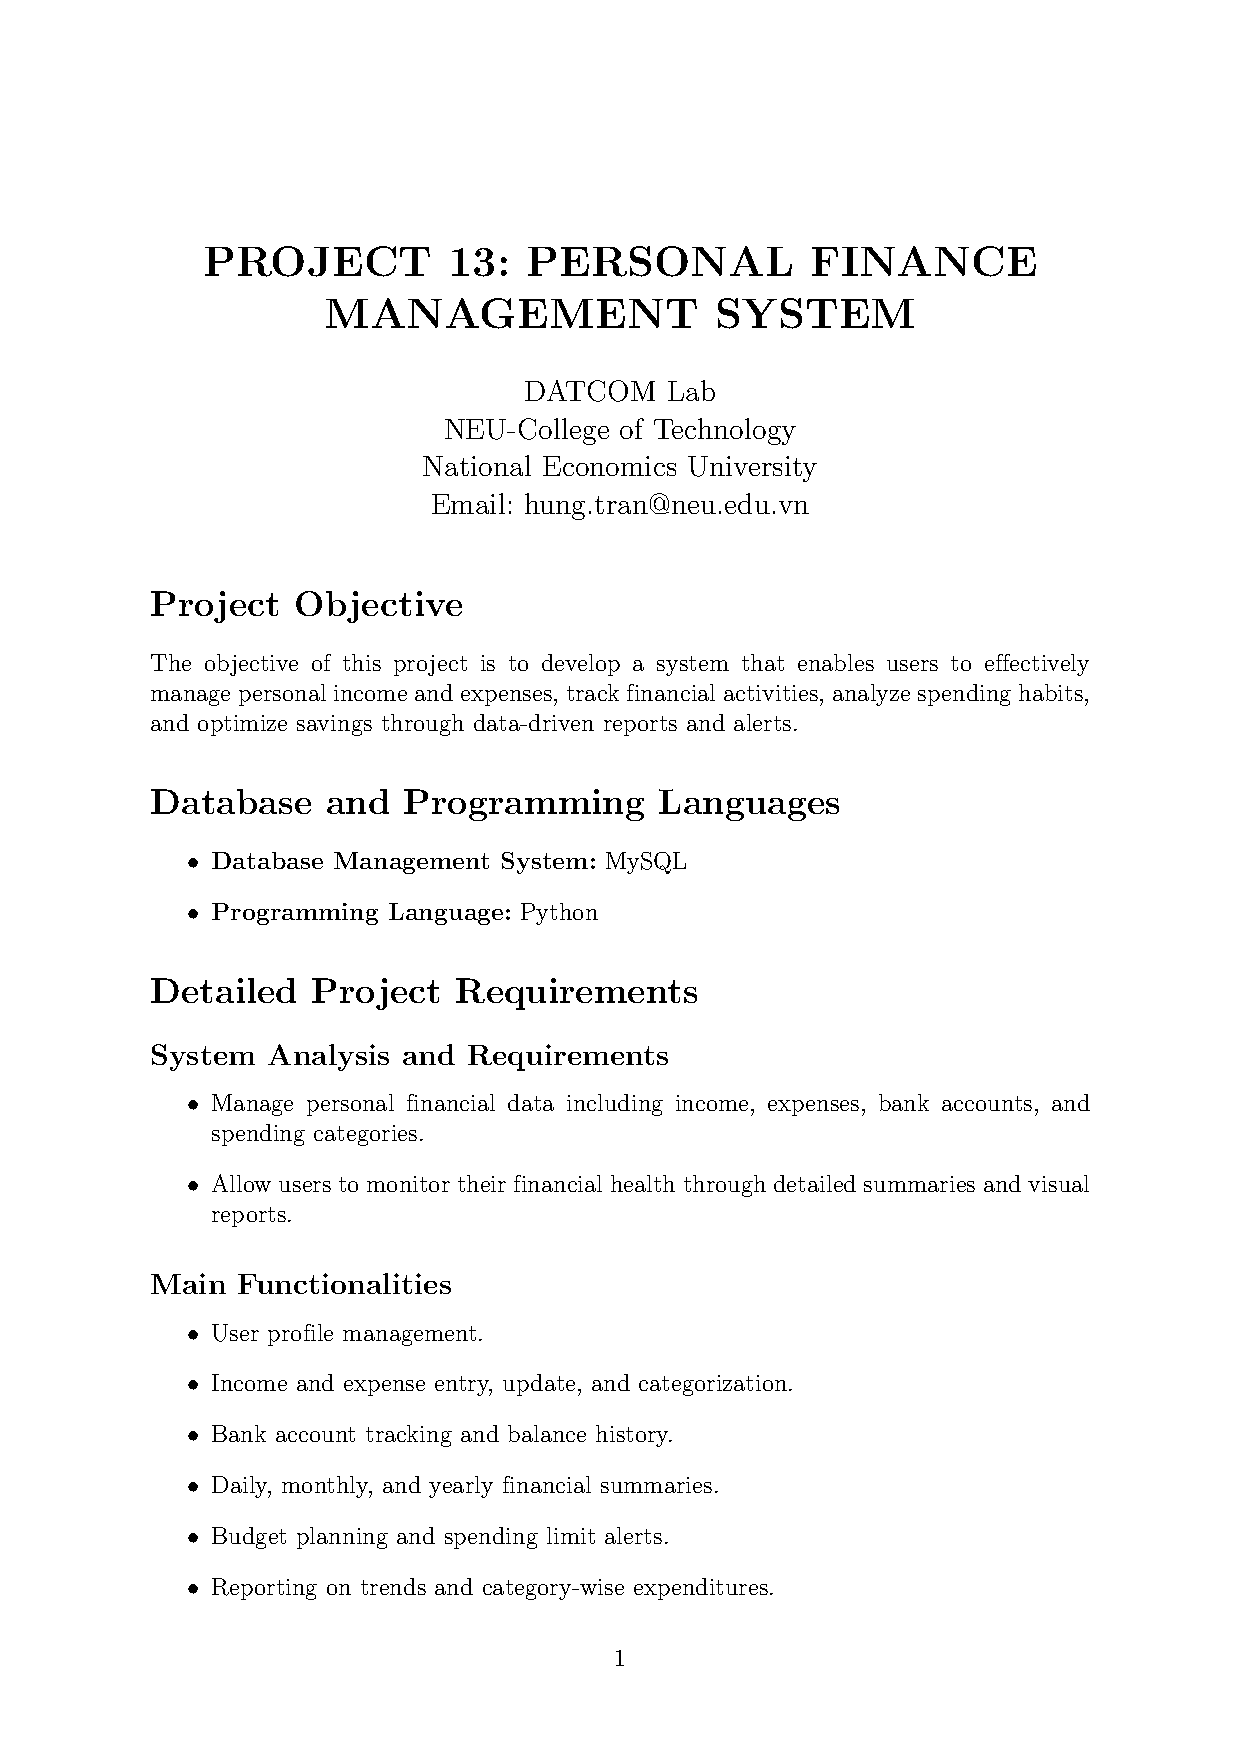
\includepdf[
    pages=-,
    pagecommand={\thispagestyle{empty}}
]{13.pdf}

\clearpage
% =========================================================
% TABLE OF CONTENTS
% =========================================================
\tableofcontents

\newpage

% =========================================================
% ABSTRACT
% =========================================================
\begin{abstract}
This report presents the design and implementation of the \projectname, a full-stack database-driven web application for managing personal financial activities. The system supports user management, authentication, bank accounts, income and expense tracking, expense categorization, monthly budget planning, fixed expenses, saving goals, goal contributions, transaction import, financial reports, and administrative functions. The database is implemented in MySQL under the schema name \dbname, while the backend is developed with FastAPI and Python, and the frontend is implemented with Next.js, TypeScript, and Tailwind CSS. The report describes the system requirements, architecture, database design, ERD diagrams, SQL implementation, backend and frontend modules, testing process, security mechanisms, limitations, and future improvements. The project demonstrates how relational database concepts such as primary keys, foreign keys, normalization, constraints, indexes, views, stored procedures, functions, and triggers can be applied to a practical personal finance management system.
\end{abstract}
% =========================================================
\section{Introduction}
% =========================================================

\subsection{Background}
Personal finance management is an important activity for individuals who want to monitor their income, control expenses, plan monthly budgets, and achieve long-term saving goals. Without a structured system, users may find it difficult to understand where their money goes, whether they are overspending, and how much they can save each month.

The \projectname{} was developed to solve this problem by providing a centralized platform for recording and analyzing personal financial data. The project focuses on database design and implementation, while also delivering a complete web application with backend APIs and a frontend user interface.

\subsection{Problem Statement}
Many users manage income and expenses manually using notes, spreadsheets, or banking applications that do not provide full financial planning functions. These methods may lack category-based spending analysis, budget warnings, saving goal tracking, transaction import, and historical reports.

This project addresses the following problems:
\begin{itemize}
    \item Users need to store personal financial data in a structured and secure database.
    \item Users need to track income and expenses by account, category, and date.
    \item Users need monthly budget planning and spending alerts.
    \item Users need to monitor saving goals and goal contributions.
    \item Users need reports and visualizations to understand financial behavior.
    \item Administrators need basic user management capabilities.
\end{itemize}

\subsection{Project Objectives}
The main objective of the project is to design and implement a relational database system for personal finance management. The specific objectives are:
\begin{itemize}
    \item Design a normalized MySQL database schema named \dbname.
    \item Implement core financial entities such as users, bank accounts, income, expenses, categories, budgets, and saving goals.
    \item Implement authentication-related tables for credentials, sessions, OTP codes, and audit logs.
    \item Implement transaction import tables for CSV/Excel import workflow.
    \item Use views, stored procedures, functions, triggers, constraints, and indexes to improve data integrity and reporting.
    \item Build a FastAPI backend to expose database operations through REST APIs.
    \item Build a Next.js frontend for user interaction and financial visualization.
    \item Deploy the system using Docker Compose locally and Railway globally.
\end{itemize}

\subsection{Project Scope}
The project scope includes both core database requirements and extended application features.

\subsubsection{Core Scope}
The core scope includes:
\begin{itemize}
    \item User profile management.
    \item Bank account management.
    \item Income and expense tracking.
    \item Expense category management.
    \item Monthly budget settings and budget plans.
    \item Saving goals and goal contributions.
    \item Financial reports and account balance history.
\end{itemize}

\subsubsection{Extended Scope}
The extended scope includes:
\begin{itemize}
    \item Authentication, session tokens, OTP, and audit logs.
    \item Admin user management.
    \item CSV/Excel transaction import.
    \item Smart budget guardrails and spending alerts.
    \item Vietnamese user interface.
    \item Railway deployment.
\end{itemize}

\subsection{Technology Stack}

\small
\renewcommand{\arraystretch}{1.15}

\begin{longtable}{
    >{\raggedright\arraybackslash}p{0.22\linewidth}
    >{\raggedright\arraybackslash}p{0.28\linewidth}
    J{0.40\linewidth}
}
\caption{Technology stack used in the project}
\label{tab:technology-stack} \\

\toprule
\textbf{Layer} & \textbf{Technology} & \textbf{Purpose} \\
\midrule
\endfirsthead

\caption[]{Technology stack used in the project (continued)} \\

\toprule
\textbf{Layer} & \textbf{Technology} & \textbf{Purpose} \\
\midrule
\endhead

\midrule
\multicolumn{3}{r}{\textit{Continued on next page}} \\
\endfoot

\bottomrule
\endlastfoot

Database 
& MySQL 
& Store relational financial data. \\

Backend 
& Python, FastAPI 
& Provide REST APIs and business logic. \\

Frontend 
& Next.js, TypeScript, Tailwind CSS 
& Build the user interface. \\

Database Driver 
& mysql-connector-python 
& Connect the backend application to MySQL. \\

Charts 
& Recharts 
& Display financial reports and visualizations. \\

Local Development 
& Docker Compose 
& Run the database, backend, and frontend locally. \\

Deployment 
& Railway 
& Host MySQL, backend, and frontend services. \\

Database Tool 
& MySQL Workbench / MySQL Query Editor 
& Run SQL commands and inspect schema, data, and query results. \\

ERD Tool 
& ERDPlus 
& Design ERD diagrams. \\

\end{longtable}

\normalsize

% =========================================================
\section{System Requirement Analysis}
% =========================================================
\subsection{Functional Requirements}

\subsubsection{User and Authentication Management}
The system must support user registration, login, logout, session management, password reset, OTP-based account unlock, and administrator-level user management. This requirement ensures that financial data is associated with the correct user and protected by authentication.

\subsubsection{Income Management}
The system must allow users to create, update, delete, and view income records. Each income transaction is linked to a user and an internally managed bank account.

\subsubsection{Expense Management}
The system must allow users to create, update, delete, and view expense records. Each expense transaction is linked to a user, a bank account, and an expense category, allowing the system to analyze spending behavior by category.

\subsubsection{Bank Account Tracking}
The system must allow users to manage self-declared bank accounts inside the application. These accounts are not connected to real banking APIs; instead, their balances are maintained internally based on income and expense transactions entered by the user.

\subsubsection{Budget Management}
The system must support monthly budget settings, fixed expense setup, category-based budget plans, planned versus actual comparison, and warning or exceeded statuses when spending approaches or exceeds the planned budget.

\subsubsection{Saving Goal Management}
The system must allow users to create saving or debt repayment goals, assign goal categories, record contributions, and monitor goal progress over time.

\subsubsection{Reporting and Visualization}
The system must provide financial reports and charts, including income versus expense summaries, category-wise spending, budget comparison, saving goal progress, account balance history, and cash flow visualization.

\subsubsection{Transaction Import}
The system must support importing transactions from CSV or Excel files. The import process includes row preview, value parsing, duplicate detection, category suggestion, and import confirmation.

\subsection{Non-functional Requirements}

\begin{itemize}
    \item \textbf{Data integrity:} The system must use primary keys, foreign keys, unique constraints, check constraints, and triggers to keep financial data consistent.
    \item \textbf{Security:} Passwords, session tokens, and OTP codes must not be stored in plain text.
    \item \textbf{Performance:} Indexes should support common lookups, dashboard queries, and financial reports.
    \item \textbf{Maintainability:} The project should separate database scripts, backend APIs, service logic, repository logic, and frontend components.
    \item \textbf{Usability:} The user interface should be clear, localized in Vietnamese, and suitable for everyday personal finance tracking.
    \item \textbf{Deployability:} The system should run locally using Docker Compose and be deployable globally using Railway.
\end{itemize}

% =========================================================
\section{System Architecture}
% =========================================================

\subsection{Overall Architecture}
The system follows a layered architecture. The user interacts with the Next.js frontend through a web browser. The frontend sends HTTP requests to the FastAPI backend through REST APIs. The backend uses a service layer to process business logic and repository classes to interact with the MySQL database.

\subsection{Repository Structure}
The project repository is organized into separate folders for database scripts, backend code, frontend code, shared Python application logic, and operational scripts.

\begin{lstlisting}[style=codestyle, caption={Main repository structure}]
database/
  schema.sql
  sample_data.sql
  views.sql
  procedures.sql
  functions.sql
  triggers.sql
  security.sql
  migrations/

backend/
frontend/
  src/
    app/
    components/
    lib/
    providers/
    types/
python_app/
ops/
docs/
docker-compose.yml
README.md
\end{lstlisting}

\subsection{Frontend Architecture}
The frontend is implemented with Next.js and TypeScript. It provides pages for login, signup, dashboard, transactions, budgets, goals, reports, balance history, profile, and user management. Tailwind CSS is used for styling, while Recharts is used for financial charts.

\subsection{Backend Architecture}
The backend is implemented with FastAPI. It exposes REST APIs under the prefix \texttt{/api/v1}. The backend includes routers for authentication, dashboard, metadata, transactions, imports, reports, budgets, alerts, goals, and user management.

\subsection{Database Architecture}
The database layer is implemented in MySQL. It includes normalized tables, constraints, indexes, views, stored procedures, user-defined functions, and triggers. The database name is fixed as \dbname.

% =========================================================
\section{Database Design}
% =========================================================

\subsection{Database Overview}

The system uses a MySQL relational database named \texttt{Personal\_Finance}.
The database stores the main financial data of the application, including users,
authentication records, bank accounts, income, expenses, budgets, saving goals,
transaction imports, sessions, OTP codes, and audit logs. The schema is designed
with primary keys, foreign keys, constraints, indexes, views, triggers, functions,
and stored procedures to ensure data consistency and support financial reporting.

\begin{table}[H]
\centering
\caption{Database overview}
\label{tab:database-overview}
\small
\renewcommand{\arraystretch}{1.15}
\begin{tabular}{ll}
\toprule
\textbf{Item} & \textbf{Description} \\
\midrule
Database name       & \texttt{Personal\_Finance} \\
DBMS                & MySQL \\
Character set       & \texttt{utf8mb4} \\
Collation           & \texttt{utf8mb4\_0900\_ai\_ci} \\
Main SQL file       & \texttt{database/schema.sql} \\
Sample data file    & \texttt{database/sample\_data.sql} \\
Views file          & \texttt{database/views.sql} \\
Stored procedures file & \texttt{database/procedures.sql} \\
Functions file      & \texttt{database/functions.sql} \\
Triggers file       & \texttt{database/triggers.sql} \\
Security setup file & \texttt{database/security.sql} \\
\bottomrule
\end{tabular}
\end{table}

\subsection{Core ERD}

The Core ERD represents the main business entities of the system.
It focuses on the tables that directly support the financial tracking workflow, including user
profiles, bank accounts, income records, expense records, budget planning, and saving goals.
These tables form the foundation of the system because most application features depend on them.

\begin{figure}[H]
    \centering
    \makebox[\textwidth][c]{%
        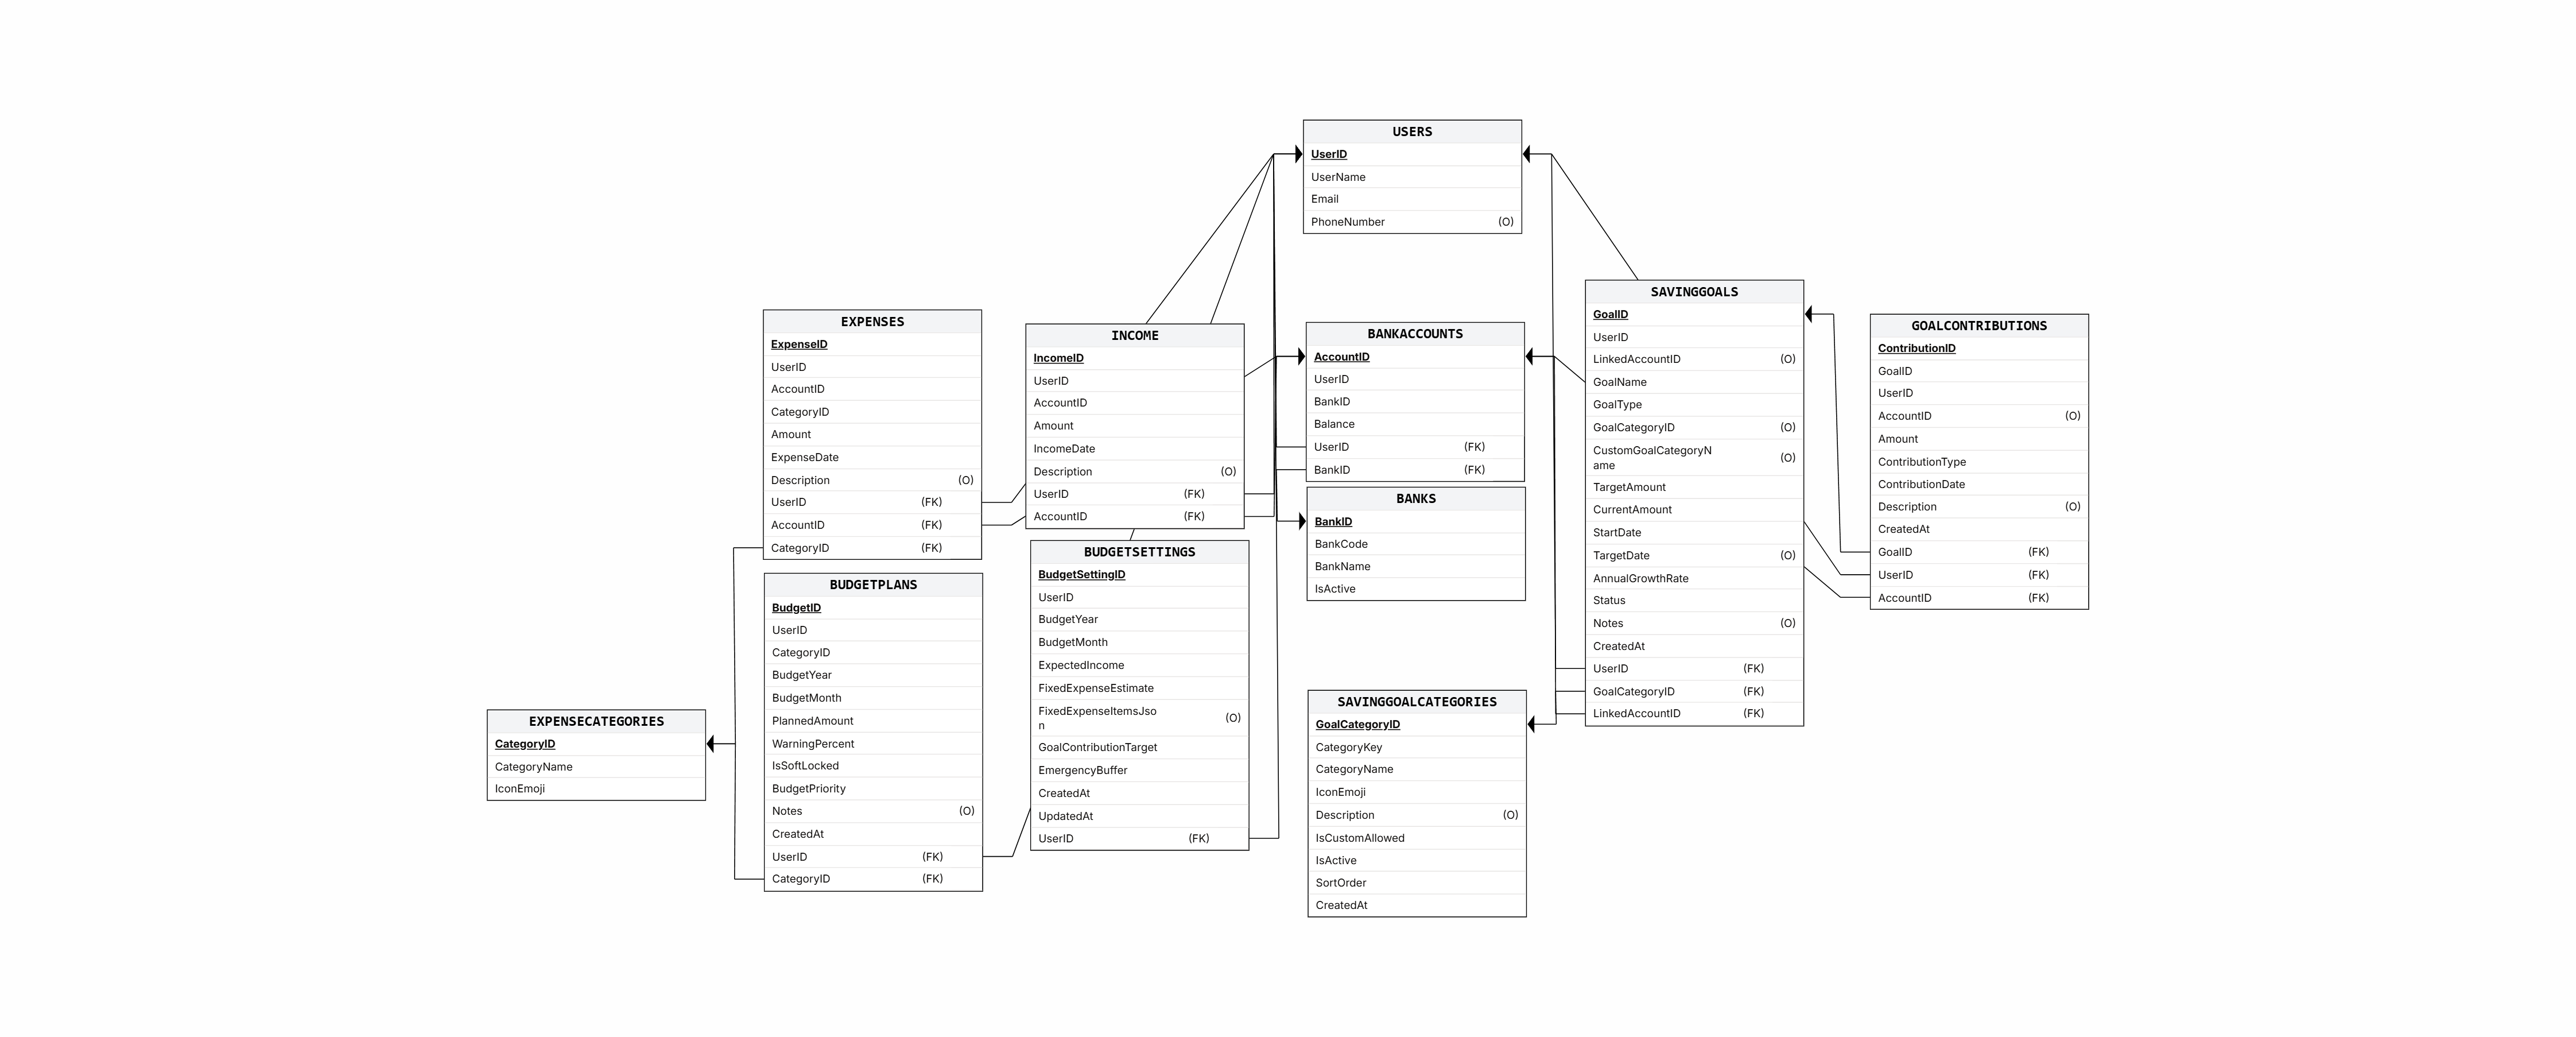
\includegraphics[width=1.5\textwidth]{ERD/core_erd.png}
    }
    \caption{Core ERD of the \dbname{} database}
    \label{fig:core-erd}
\end{figure}

The core database design is organized around the \texttt{Users} table. Each user can own multiple
bank accounts, record income and expense transactions, create monthly budgets, and define saving
or debt repayment goals. This user-centered design ensures that all financial records are clearly
separated by account owner.

\subsubsection{Core Entities}

\begin{longtable}{
    >{\raggedright\arraybackslash}p{0.28\linewidth}
    J{0.62\linewidth}
}
\caption{Core entities in the database}
\label{tab:core-entities} \\

\toprule
\textbf{Entity} & \textbf{Purpose} \\
\midrule
\endfirsthead

\caption[]{Core entities in the database (continued)} \\

\toprule
\textbf{Entity} & \textbf{Purpose} \\
\midrule
\endhead

\midrule
\multicolumn{2}{r}{\textit{Continued on next page}} \\
\endfoot

\bottomrule
\endlastfoot

\texttt{Users}               & Stores user profile information. \\
\texttt{Banks}               & Stores the predefined bank catalog, normalized separately from user accounts. \\
\texttt{BankAccounts}        & Stores user-created bank accounts and their current balances. \\
\texttt{Income}              & Stores income transactions. \\
\texttt{Expenses}            & Stores expense transactions. \\
\texttt{ExpenseCategories}   & Stores expense categories. \\
\texttt{BudgetSettings}      & Stores monthly budget settings per user. \\
\texttt{BudgetPlans}         & Stores category-based budget plans per user per month. \\
\texttt{SavingGoalCategories}& Stores predefined saving goal categories and indicates whether custom goal category names are allowed. \\
\texttt{SavingGoals}         & Stores saving and debt repayment goals. \\
\texttt{GoalContributions}   & Stores individual contributions toward saving goals. \\

\end{longtable}

\subsubsection{Core Relationships}

The relationships in the Core ERD are designed to preserve ownership and financial consistency.
The \texttt{Users} table has one-to-many relationships with most financial tables because each
user can manage multiple accounts, transactions, budgets, and goals. The \texttt{BankAccounts}
table acts as a central link between users and transactions because income and expenses must be
assigned to a specific account. Expense transactions are also classified by \texttt{ExpenseCategories},
which allows the system to generate category-wise spending reports.

\small
\renewcommand{\arraystretch}{1.2}

\begin{longtable}{
    >{\raggedright\arraybackslash}p{0.30\linewidth}
    >{\centering\arraybackslash}p{0.18\linewidth}
    J{0.42\linewidth}
}
\caption{Main relationships in the Core ERD}
\label{tab:core-relationships} \\

\toprule
\textbf{Relationship} & \textbf{Cardinality} & \textbf{Description} \\
\midrule
\endfirsthead

\caption[]{Main relationships in the Core ERD (continued)} \\

\toprule
\textbf{Relationship} & \textbf{Cardinality} & \textbf{Description} \\
\midrule
\endhead

\midrule
\multicolumn{3}{r}{\textit{Continued on next page}} \\
\endfoot

\bottomrule
\endlastfoot

\texttt{Users -- BankAccounts}
    & One-to-many
    & One user can create multiple internal bank accounts. \\

\texttt{Banks -- BankAccounts}
    & One-to-many
    & One bank entry in the catalog can be referenced by multiple user accounts. \\

\texttt{Users -- Income}
    & One-to-many
    & One user can record multiple income transactions. \\

\texttt{Users -- Expenses}
    & One-to-many
    & One user can record multiple expense transactions. \\

\texttt{BankAccounts -- Income}
    & One-to-many
    & Each income transaction is credited to one bank account. \\

\texttt{BankAccounts -- Expenses}
    & One-to-many
    & Each expense transaction is deducted from one bank account. \\

\texttt{ExpenseCategories -- Expenses}
    & One-to-many
    & One category can classify many expense transactions. \\

\texttt{Users -- BudgetSettings}
    & One-to-many
    & One user can configure monthly budget settings across multiple months. \\

\texttt{Users -- BudgetPlans}
    & One-to-many
    & One user can define multiple category-level budget plans. \\

\texttt{ExpenseCategories -- BudgetPlans}
    & One-to-many
    & Each budget plan is assigned to one expense category. \\

\texttt{Users -- SavingGoals}
    & One-to-many
    & One user can create multiple saving or debt repayment goals. \\

\texttt{Users -- GoalContributions}
    & One-to-many
    & One user can create multiple contribution records toward saving goals. \\

\texttt{SavingGoals -- GoalContributions}
    & One-to-many
    & One goal can receive multiple contribution records over time. \\

\texttt{BankAccounts -- GoalContributions}
    & Optional one-to-many
    & A goal contribution can optionally be associated with one bank account. \\

\end{longtable}
\normalsize

\subsubsection{Design Rationale}

The Core ERD separates the main financial data into clear business entities to reduce redundancy
and improve data consistency. The \texttt{Income} and \texttt{Expenses} tables are stored separately
because they represent opposite types of transactions. Income records increase account balances,
while expense records decrease them. This separation also makes transaction processing and
financial reporting easier to understand.

The \texttt{ExpenseCategories} table is separated from \texttt{Expenses} to avoid storing repeated
category names in every expense record. This design supports category-based analysis, such as
identifying which types of expenses take the largest portion of a user's spending. Similarly,
the budget module is divided into \texttt{BudgetSettings} and \texttt{BudgetPlans}.
\texttt{BudgetSettings} stores the monthly budget configuration for each user, while
\texttt{BudgetPlans} stores planned amounts for specific expense categories.

Regarding bank account modeling, the project requirement specification defined
\texttt{BankAccounts} as a single table containing a \texttt{BankName} attribute. In this
implementation, however, bank information is normalized into a separate \texttt{Banks} table,
with \texttt{BankAccounts} referencing \texttt{Banks} via a \texttt{BankID} foreign key. This
design decision eliminates the repetition of bank names across multiple user accounts, satisfies
the Third Normal Form (3NF), and allows the application to maintain a controlled catalog of
supported banks while still associating each user account with the correct institution.

The saving goal feature is modeled separately from daily transactions because saving goals
represent long-term financial objectives. The \texttt{SavingGoals} table stores the goal
information, while \texttt{GoalContributions} stores each contribution made toward a goal. This
allows the system to calculate progress and monitor whether users are moving toward their
financial targets.

Overall, the Core ERD provides a normalized and maintainable structure for the main financial
features of the application. It supports income and expense tracking, internal bank account
balance management, monthly budgeting, saving goal monitoring, and financial reporting.

% -------------------------------------------------------------------------
\subsection{Authentication and Security Supporting ERD}
% -------------------------------------------------------------------------

The Authentication and Security Supporting ERD describes the database structure used to support
application-level authentication, account protection, OTP verification, audit logging, and session
management. Although these tables are not directly related to daily financial transactions, they are
important because they protect user accounts and ensure that financial data can only be accessed by
authorized users.

\begin{figure}[H]
    \centering
    \makebox[\textwidth][c]{%
        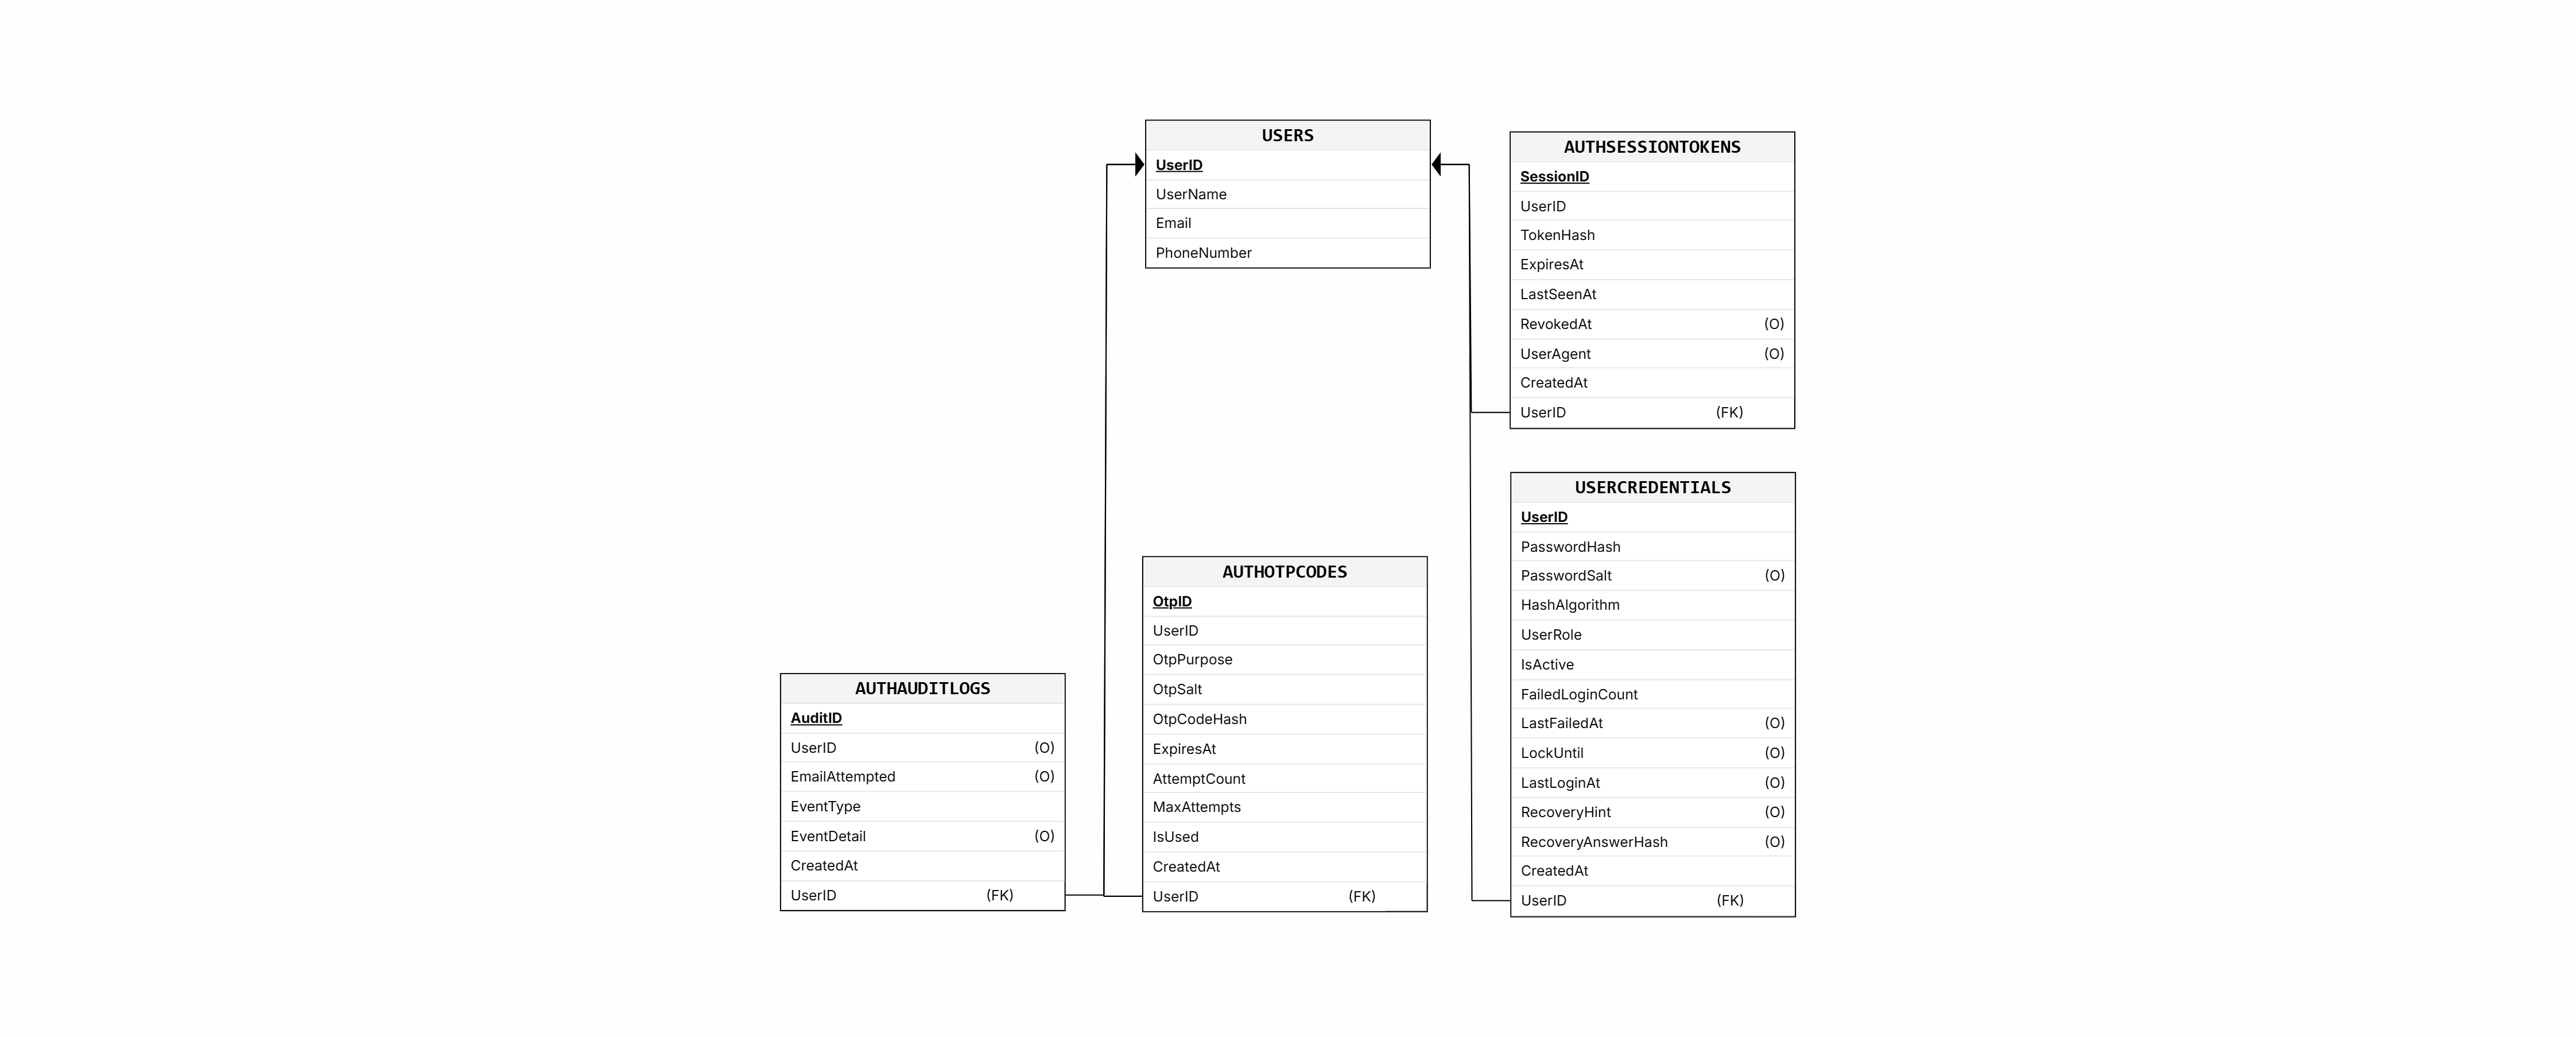
\includegraphics[width=1.5\textwidth]{ERD/auth_security_erd.png}
    }
    \caption{Authentication and Security Supporting ERD}
    \label{fig:auth-security-erd}
\end{figure}

The authentication design is centered around the \texttt{Users} table. The \texttt{Users} table
stores basic profile information, while security-sensitive information is separated into supporting
tables. This separation helps keep user profile data independent from login credentials, session
tokens, OTP codes, and audit logs.

\subsubsection{Authentication and Security Entities}

\begin{longtable}{
    >{\raggedright\arraybackslash}p{0.28\linewidth}
    J{0.62\linewidth}
}
\caption{Authentication and security supporting entities}
\label{tab:auth-security-entities} \\

\toprule
\textbf{Entity} & \textbf{Purpose} \\
\midrule
\endfirsthead

\caption[]{Authentication and security supporting entities (continued)} \\

\toprule
\textbf{Entity} & \textbf{Purpose} \\
\midrule
\endhead

\midrule
\multicolumn{2}{r}{\textit{Continued on next page}} \\
\endfoot

\bottomrule
\endlastfoot

\texttt{Users}
& Stores basic user profile information. \\

\texttt{UserCredentials}
& Stores login credentials, roles, account status, and recovery information. \\

\texttt{AuthOtpCodes}
& Stores hashed OTP codes for password reset and account unlock workflows. \\

\texttt{AuthAuditLogs}
& Stores authentication-related audit events. \\

\texttt{AuthSessionTokens}
& Stores hashed session tokens for authenticated user sessions. \\

\end{longtable}

\subsubsection{Authentication and Security Relationships}

Most supporting security records are linked to \texttt{Users} through the \texttt{UserID} foreign
key. However, \texttt{AuthAuditLogs.UserID} may be nullable when recording failed login attempts
or authentication events for unknown or unmatched email addresses. The relationship between
\texttt{Users} and \texttt{UserCredentials} is one-to-one because each user should have one
credential record. Other tables such as \texttt{AuthOtpCodes} and \texttt{AuthSessionTokens}
have one-to-many relationships with \texttt{Users}, because one user can request multiple OTP
codes and own multiple session tokens over time. \texttt{AuthAuditLogs} can also store many
records for one user when the user is known, while still allowing unauthenticated or unmatched
attempts to be logged.

\begin{longtable}{
    >{\raggedright\arraybackslash}p{0.32\linewidth}
    >{\centering\arraybackslash}p{0.18\linewidth}
    J{0.42\linewidth}
}
\caption{Main relationships in the Authentication and Security ERD}
\label{tab:auth-security-relationships} \\

\toprule
\textbf{Relationship} & \textbf{Cardinality} & \textbf{Description} \\
\midrule
\endfirsthead

\caption[]{Main relationships in the Authentication and Security ERD (continued)} \\

\toprule
\textbf{Relationship} & \textbf{Cardinality} & \textbf{Description} \\
\midrule
\endhead

\midrule
\multicolumn{3}{r}{\textit{Continued on next page}} \\
\endfoot

\bottomrule
\endlastfoot

\texttt{Users -- UserCredentials}
& One-to-one
& Each user has exactly one credential record storing password hash, role, and account status. \\

\texttt{Users -- AuthOtpCodes}
& One-to-many
& One user can request multiple OTP codes for password reset or account unlock operations. \\

\texttt{Users -- AuthAuditLogs}
& Optional one-to-many
& One known user can generate multiple authentication audit log records, while some audit logs may store only the attempted email. \\

\texttt{Users -- AuthSessionTokens}
& One-to-many
& One user can hold multiple session tokens, for example when authenticated across different devices or browsers. \\

\end{longtable}

\subsubsection{Design Rationale}

The authentication and security tables are separated from the core financial tables to improve
security, maintainability, and clarity. The \texttt{Users} table stores general profile information,
while \texttt{UserCredentials} stores sensitive login-related data such as password hashes, user
roles, account status, and recovery information.

The system avoids storing sensitive authentication data in plain text. Passwords, OTP codes, and
session tokens are stored as hashes or salted hashes to reduce security risks if the database is
accessed improperly.

The \texttt{AuthOtpCodes} table supports temporary verification workflows such as password reset
and account unlocking. The \texttt{AuthSessionTokens} table manages authenticated sessions by
tracking token expiration, last activity, and revocation status.

The \texttt{AuthAuditLogs} table records important authentication events, such as failed login
attempts, account lock actions, password reset requests, and OTP-related activities.

Overall, this supporting ERD strengthens the authentication layer and provides traceability for
account-related events.

% -------------------------------------------------------------------------
\subsection{Transaction Import and Linking Supporting ERD}
% -------------------------------------------------------------------------

The Transaction Import and Linking Supporting ERD describes the database structure used to support
CSV/Excel transaction import, automatic category suggestion, duplicate detection, import
confirmation, and the linking between financial transactions and saving goal contributions. This
ERD extends the core financial model by adding supporting tables that help users import external
transaction data and connect income or expense transactions with long-term financial goals.

\begin{figure}[H]
    \centering
    \makebox[\textwidth][c]{%
        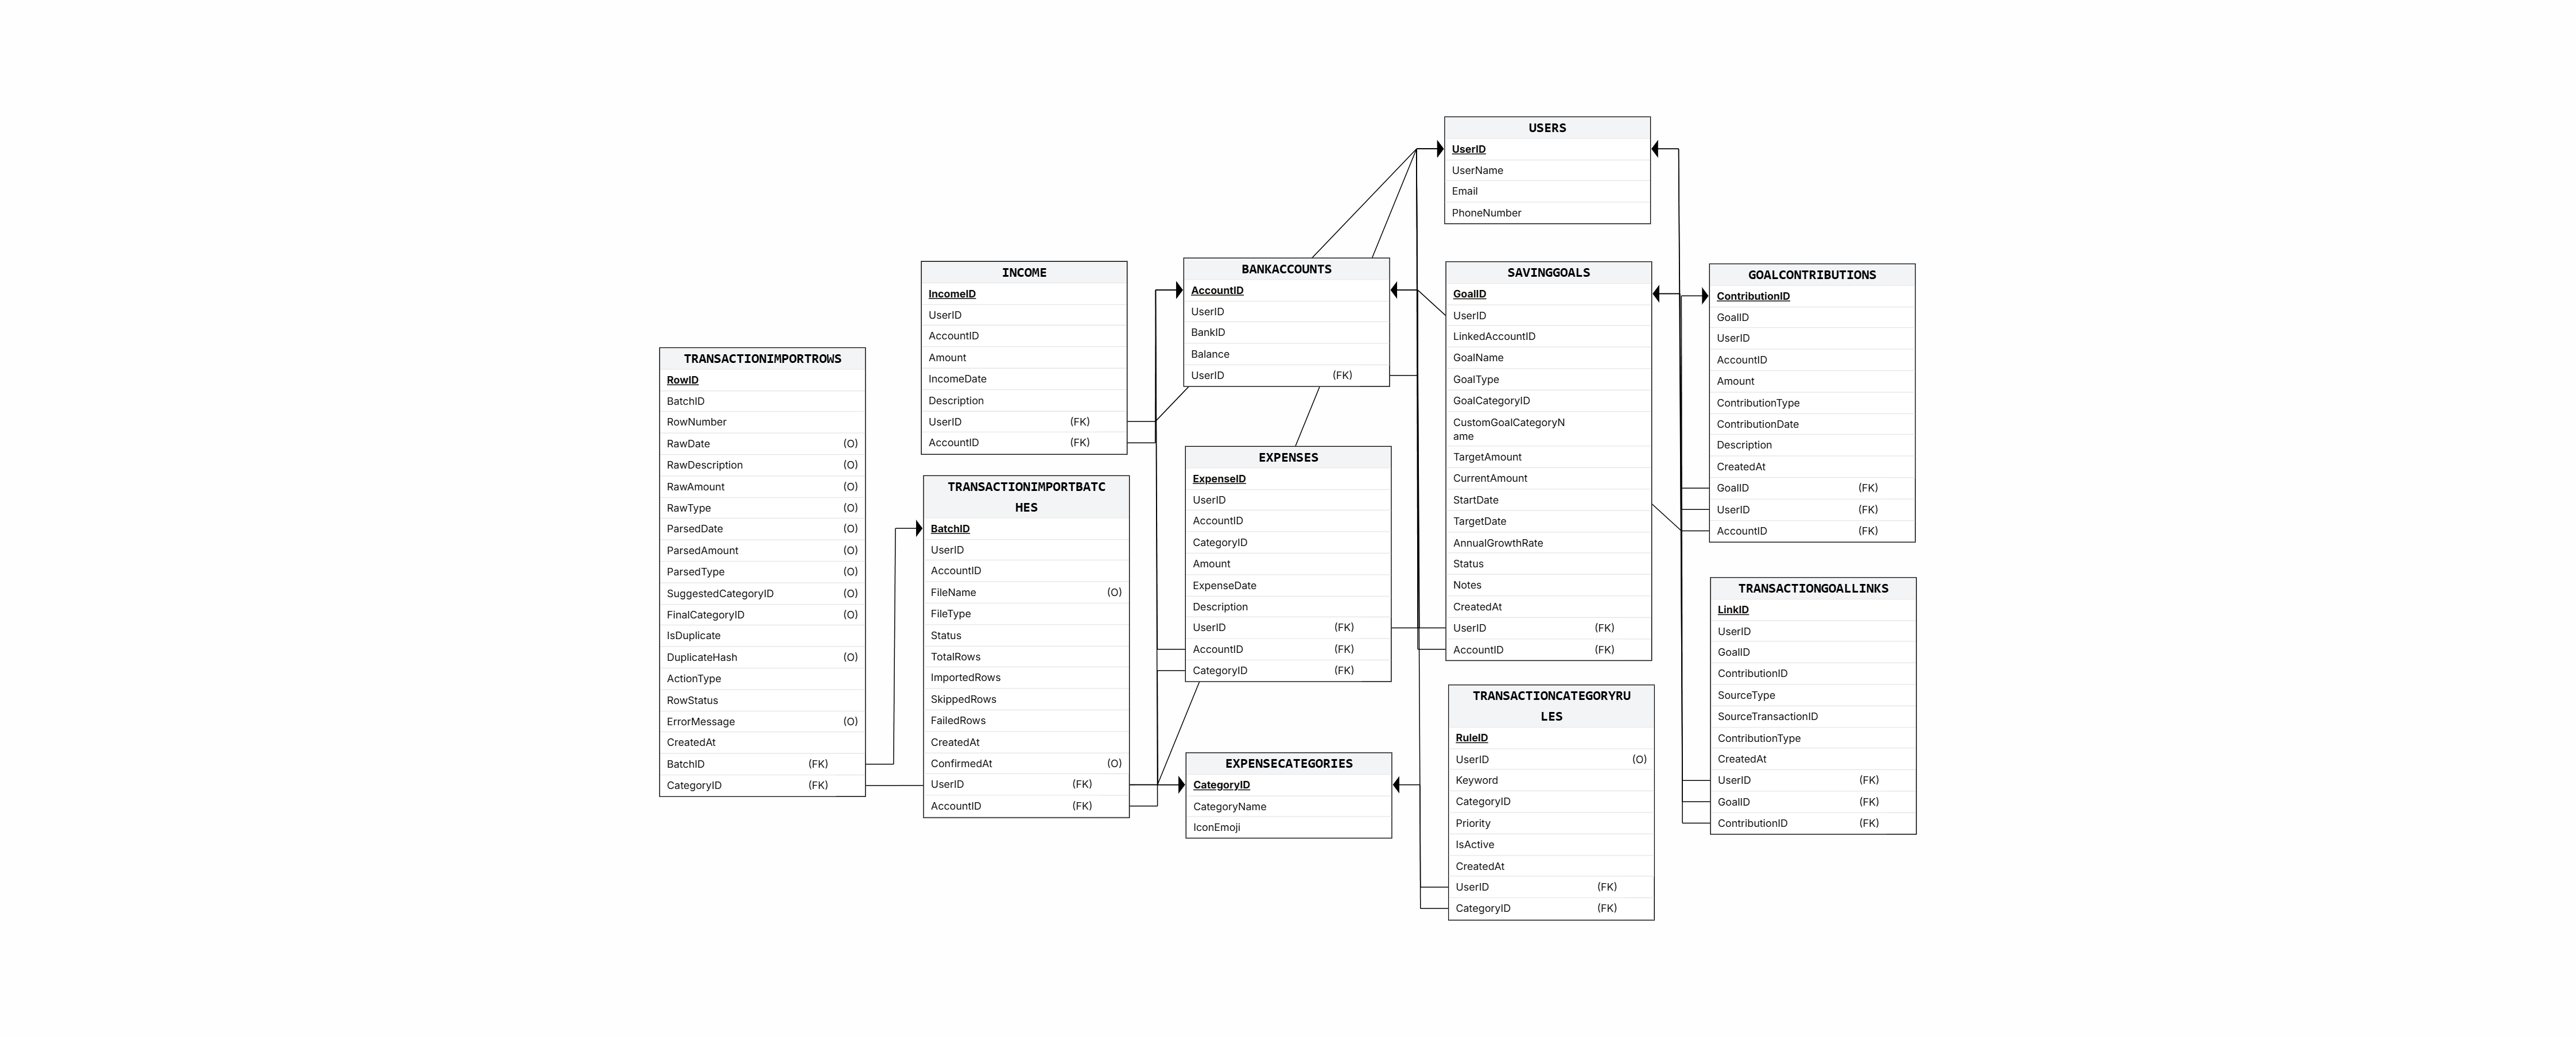
\includegraphics[width=1.5\textwidth]{ERD/transaction_erd.png}
    }
    \caption{Transaction Import and Linking Supporting ERD}
    \label{fig:transaction-import-linking-erd}
\end{figure}

This supporting ERD is built around the transaction workflow. The import process starts with a
file uploaded by the user. The file is stored as an import batch in
\texttt{TransactionImportBatches}, while each row of the file is stored in
\texttt{TransactionImportRows}. The system can parse raw transaction data, suggest categories
based on predefined rules, detect duplicate transactions, and allow the user to confirm the
final import action. In addition, the \texttt{TransactionGoalLinks} table records the
relationship between imported or manually entered transactions and goal contributions.

\subsubsection{Transaction Import and Linking Entities}

\begin{longtable}{
    >{\raggedright\arraybackslash}p{0.30\linewidth}
    J{0.60\linewidth}
}
\caption{Transaction import and linking supporting entities}
\label{tab:transaction-import-linking-entities} \\

\toprule
\textbf{Entity} & \textbf{Purpose} \\
\midrule
\endfirsthead

\caption[]{Transaction import and linking supporting entities (continued)} \\

\toprule
\textbf{Entity} & \textbf{Purpose} \\
\midrule
\endhead

\midrule
\multicolumn{2}{r}{\textit{Continued on next page}} \\
\endfoot

\bottomrule
\endlastfoot

\texttt{TransactionImportBatches}
& Stores file-level information for each CSV or Excel import. \\

\texttt{TransactionImportRows}
& Stores row-level transaction data during the import process. \\

\texttt{TransactionCategoryRules}
& Stores keyword rules used to suggest expense categories. \\

\texttt{TransactionGoalLinks}
& Links income or expense transactions with goal contributions, enabling traceability between daily
financial activities and long-term financial goals. \\

\texttt{Income}
& Stores income transactions. \\

\texttt{Expenses}
& Stores expense transactions. \\

\texttt{SavingGoals}
& Stores saving or debt repayment goals. \\

\texttt{GoalContributions}
& Stores contribution records toward saving goals. \\

\texttt{Users}
& Stores the owner of transactions, imports, rules, and goals. \\

\texttt{BankAccounts}
& Stores the bank account associated with transactions and imports. \\

\texttt{ExpenseCategories}
& Stores categories used to classify expense transactions. \\

\end{longtable}

\subsubsection{Transaction Import and Linking Relationships}

The transaction import workflow is user-centered. Each import batch belongs to one user and one
bank account. Each batch contains multiple import rows, and each import row can be parsed,
categorized, marked as duplicate, skipped, failed, or confirmed for import. Category suggestion
is supported by \texttt{TransactionCategoryRules}, which map user-defined keywords to
\texttt{ExpenseCategories}.

The linking workflow connects normal financial transactions with saving goal contributions. A
record in \texttt{TransactionGoalLinks} connects one source transaction to one goal contribution.
The source transaction may come from either \texttt{Income} or \texttt{Expenses}, depending on the
value of \texttt{SourceType}.

\begin{longtable}{
    >{\raggedright\arraybackslash}p{0.34\linewidth}
    >{\centering\arraybackslash}p{0.18\linewidth}
    J{0.38\linewidth}
}
\caption{Main relationships in the Transaction Import and Linking ERD}
\label{tab:transaction-import-linking-relationships} \\

\toprule
\textbf{Relationship} & \textbf{Cardinality} & \textbf{Description} \\
\midrule
\endfirsthead

\caption[]{Main relationships in the Transaction Import and Linking ERD (continued)} \\

\toprule
\textbf{Relationship} & \textbf{Cardinality} & \textbf{Description} \\
\midrule
\endhead

\midrule
\multicolumn{3}{r}{\textit{Continued on next page}} \\
\endfoot

\bottomrule
\endlastfoot

\texttt{Users -- TransactionImportBatches}
& One-to-many
& One user can create multiple transaction import batches. \\

\texttt{BankAccounts -- TransactionImportBatches}
& One-to-many
& One bank account can be associated with multiple imported transaction files. \\

\texttt{TransactionImportBatches -- TransactionImportRows}
& One-to-many
& One import batch contains multiple imported rows from the uploaded file. \\

\texttt{ExpenseCategories -- TransactionImportRows}
& One-to-many
& One expense category can be used as the suggested or final category for many imported rows. \\

\texttt{Users -- TransactionCategoryRules}
& One-to-many
& One user can define multiple keyword-based category rules. \\

\texttt{ExpenseCategories -- TransactionCategoryRules}
& One-to-many
& One expense category can be referenced by multiple category suggestion rules. \\

\texttt{Users -- TransactionGoalLinks}
& One-to-many
& One user can have multiple links between transactions and goal contributions. \\

\texttt{SavingGoals -- TransactionGoalLinks}
& One-to-many
& One saving goal can be linked to multiple transaction-related contributions. \\

\texttt{GoalContributions -- TransactionGoalLinks}
& Optional one-to-one
& Each transaction-goal link refers to exactly one goal contribution, while a manual contribution may exist without a transaction-goal link. \\

\texttt{Income -- TransactionGoalLinks}
& Conditional
& If \texttt{SourceType = INCOME}, then \texttt{SourceTransactionID} refers to \texttt{Income.IncomeID}. \\

\texttt{Expenses -- TransactionGoalLinks}
& Conditional
& If \texttt{SourceType = EXPENSE}, then \texttt{SourceTransactionID} refers to \texttt{Expenses.ExpenseID}. \\

\end{longtable}

\textbf{Special Notes}

\begin{itemize}
    \item \textbf{Polymorphic reference in \texttt{TransactionGoalLinks}:}
    \texttt{SourceTransactionID} can refer to either \texttt{Income.IncomeID} or
    \texttt{Expenses.ExpenseID}, depending on the value of \texttt{SourceType}.
    Because MySQL does not natively support polymorphic foreign keys, this relationship
    must be validated at the backend application layer.

    \item \textbf{Optional category references in \texttt{TransactionImportRows}:}
    \texttt{SuggestedCategoryID} stores the category proposed by the system via keyword
    matching, while \texttt{FinalCategoryID} stores the category confirmed by the user
    before import. Both fields reference \texttt{ExpenseCategories.CategoryID} and are
    nullable to allow rows where no category has yet been assigned.

    \item \textbf{Duplicate detection:}
    \texttt{IsDuplicate} and \texttt{DuplicateHash} are used to detect repeated imported
    transactions and prevent the creation of duplicate financial records.
\end{itemize}

\subsubsection{Design Rationale}

The transaction import design separates file-level data from row-level data to make the import
process easier to control. A batch represents one uploaded file, while each row can be reviewed,
corrected, skipped, or confirmed independently. This structure allows the system to track both the
overall import status and the detailed outcome of each imported transaction row.

The category rule mechanism is included to reduce manual effort during transaction import. By
matching transaction descriptions against user-defined keywords stored in
\texttt{TransactionCategoryRules}, the system can propose suitable expense categories before the
user confirms the final classification.

The transaction-goal linking design improves traceability between daily financial activities and
long-term saving objectives. Rather than embedding goal-related logic directly within the
\texttt{Income} or \texttt{Expenses} tables, the system stores these associations in the separate
\texttt{TransactionGoalLinks} table. This approach preserves the integrity of core transaction
records while still allowing the system to identify which financial transaction contributed to a
specific saving or debt repayment goal.

Overall, this supporting ERD improves the import workflow, reduces duplicate transaction records,
supports automatic category suggestion, and maintains a clear and auditable connection between
transactions and saving goals.

% -------------------------------------------------------------------------
\subsection{Full ERD}
% -------------------------------------------------------------------------

The Full ERD contains all nineteen tables in the \texttt{Personal\_Finance} database. Because it
is larger and more detailed than the individual supporting diagrams, it is placed in
Appendix~\ref{appendix:full-erd} for reference.

% -------------------------------------------------------------------------
\subsection{Normalization}
% -------------------------------------------------------------------------

The database schema follows normalization principles to reduce redundancy, avoid update anomalies, and improve data consistency. The design is organized so that each table stores one main type of data and relationships are represented through primary keys and foreign keys.

\subsubsection{First Normal Form (1NF)}

The schema satisfies First Normal Form because table attributes store atomic values and each record is uniquely identified by a primary key. For example, \texttt{Users} stores one user per row, \texttt{Income} stores one income transaction per row, and \texttt{Expenses} stores one expense transaction per row. Repeating groups are avoided by separating related data into different tables instead of storing multiple values in one column.

\subsubsection{Second Normal Form (2NF)}

The schema satisfies Second Normal Form because non-key attributes depend on the whole primary key of their table. Most tables use a single surrogate primary key, such as \texttt{UserID}, \texttt{IncomeID}, \texttt{ExpenseID}, or \texttt{GoalID}, which reduces the risk of partial dependency. Relationship data is stored through foreign keys. For example, \texttt{Income} and \texttt{Expenses} reference \texttt{Users} and \texttt{BankAccounts} instead of repeating user or account details inside transaction records.

\subsubsection{Third Normal Form (3NF)}

The schema satisfies Third Normal Form because non-key attributes do not depend on other non-key attributes. Lookup and supporting data are separated into independent tables. For example, bank catalog information is stored in \texttt{Banks}, while user-owned accounts are stored in \texttt{BankAccounts}. Expense category names are stored in \texttt{ExpenseCategories}, while expense records only reference the category through \texttt{CategoryID}. Similarly, \texttt{Users} stores general profile data, while \texttt{UserCredentials} stores authentication-related data.

Overall, the normalization design keeps the schema clean and maintainable. It reduces repeated values, improves consistency, and allows the system to manage financial transactions, budgets, goals, authentication, and reports more reliably.

% -------------------------------------------------------------------------
\subsection{Constraints and Data Integrity}
% -------------------------------------------------------------------------

The database uses several integrity mechanisms to ensure that financial data remains accurate and consistent.

\begin{itemize}
    \item \textbf{Primary keys} uniquely identify records in each table. Most tables use a numeric 
    auto-incremented key, such as \texttt{UserID}, \texttt{IncomeID}, or \texttt{ExpenseID}.

    \item \textbf{Foreign keys} enforce relationships between related tables. For example, expense records 
    are linked to users, bank accounts, and expense categories.

    \item \textbf{Unique constraints} prevent duplicate important values, such as user emails, phone numbers, 
    bank codes, bank names, and repeated monthly budget plans for the same user and category.

    \item \textbf{Check constraints} enforce valid financial values and period values, such as positive 
    transaction amounts, non-negative balances, valid warning percentages, and valid budget months.

    \item \textbf{Triggers} keep \texttt{BankAccounts.Balance} synchronized when income or expense records 
    are inserted, updated, or deleted. They also help prevent expense transactions when the selected account 
    does not have enough balance.
\end{itemize}

Together, these mechanisms protect the database from invalid records and help maintain reliable financial data.

% -------------------------------------------------------------------------
\subsection{Indexing Strategy}
% -------------------------------------------------------------------------

Indexes are created to improve query performance for the most common access patterns in the application. 
Because most features are user-scoped and time-scoped, the indexing strategy prioritizes composite 
indexes on \texttt{UserID} combined with relevant date, period, status, or lookup columns.

\begin{itemize}
    \item \textbf{Transaction reporting:} 
    Indexes such as \path{Income(UserID,IncomeDate)} and 
    \path{Expenses(UserID,ExpenseDate)} support dashboard and monthly summary queries. 
    Additional indexes on \path{Income(IncomeDate)} and 
    \path{Expenses(ExpenseDate,CategoryID)} support cross-user reporting and category-wise 
    spending analysis.

    \item \textbf{Budget management:} 
    Indexes on \path{BudgetPlans(UserID,BudgetYear,BudgetMonth)} and 
    \path{BudgetSettings(UserID,BudgetYear,BudgetMonth)} support monthly budget lookups. 
    An additional index on \path{BudgetPlans(UserID,BudgetYear,BudgetMonth,IsSoftLocked,BudgetPriority)} 
    supports filtered retrieval of locked or high-priority budget lines.

    \item \textbf{Authentication and sessions:} 
    Indexes on \path{AuthSessionTokens(UserID,ExpiresAt)} and 
    \path{AuthSessionTokens(ExpiresAt,RevokedAt)} support session validation and expired-session cleanup. 
    OTP-related indexes support OTP lookup, expiry checks, and audit trail retrieval.

    \item \textbf{Saving goals and contributions:} 
    Indexes on \path{SavingGoals(UserID,Status)}, \path{SavingGoals(UserID,TargetDate)}, 
    and \path{GoalContributions(GoalID,ContributionDate)} support goal progress queries and 
    contribution history lookup.

    \item \textbf{Transaction import:} 
    Indexes on \path{TransactionImportBatches(UserID,CreatedAt)}, 
    \path{TransactionImportRows(BatchID,RowNumber)}, and 
    \path{TransactionImportRows(DuplicateHash)} support batch retrieval, row-by-row access, 
    and duplicate detection during file import.
\end{itemize}

Overall, the indexing strategy is aligned with the main query patterns of the system, including 
dashboard loading, financial reporting, budget analysis, session validation, goal tracking, and 
transaction import.

% =========================================================
\section{SQL Implementation}
\label{sec:sql-implementation}
% =========================================================

This section describes the SQL implementation of the \texttt{Personal\_Finance} database. 
The implementation is divided into several SQL files, including \texttt{schema.sql}, 
\texttt{sample\_data.sql}, \texttt{views.sql}, \texttt{procedures.sql}, 
\texttt{functions.sql}, \texttt{triggers.sql}, \texttt{security.sql}, and the 
\texttt{migrations/} folder. These files define the database structure, insert sample data, 
create reporting views, implement stored routines, automate account balance updates, and 
configure database-level access control.

The screenshots in this chapter are captured from MySQL query results. Each screenshot is 
shown together with the SQL command used to produce it.

% -------------------------------------------------------------------------
\subsection{Schema Implementation}
% -------------------------------------------------------------------------

The main schema is defined in \texttt{database/schema.sql}. This file creates the 
\texttt{Personal\_Finance} database and defines the main relational structure of the system. 
It includes tables, primary keys, foreign keys, unique constraints, check constraints, and 
indexes. The schema covers user management, authentication, bank accounts, income, expenses, 
budgets, saving goals, transaction import, sessions, OTP verification, and audit logging.

Most tables use a numeric auto-incremented surrogate primary key. The main exception is 
\texttt{UserCredentials}, which uses \texttt{UserID} as both its primary key and foreign key 
to \texttt{Users}. Foreign key constraints are used to maintain relationships between related 
tables. In addition, \path{BankAccounts(AccountID,UserID)} is used as a composite unique key 
to ensure that transactions are linked only to accounts owned by the correct user.

The following SQL command was used to verify the created tables and views:

\begin{lstlisting}[style=sqlstyle]
USE Personal_Finance;

SHOW FULL TABLES;
\end{lstlisting}

\begin{figure}[H]
    \centering

    \begin{subfigure}[t]{0.35\textwidth}
        \centering
        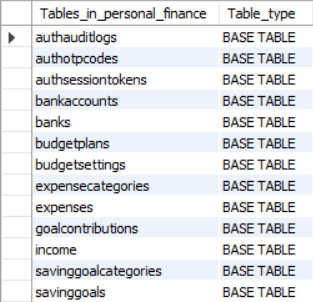
\includegraphics[width=\linewidth]{figures/full_table.png}
        \caption{Base tables}
        \label{fig:sql-full-table-1}
    \end{subfigure}
    \hspace{-0.02\textwidth}
    \begin{subfigure}[t]{0.35\textwidth}
        \centering
        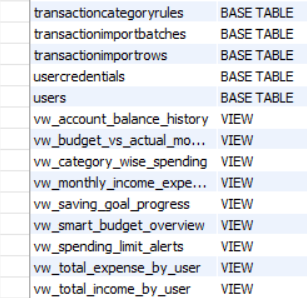
\includegraphics[width=\linewidth]{figures/full_table_2.png}
        \caption{Remaining tables and views}
        \label{fig:sql-full-table-2}
    \end{subfigure}

    \caption{MySQL result of \texttt{SHOW FULL TABLES} in the \texttt{Personal\_Finance} database}
    \label{fig:sql-show-full-tables}
\end{figure}

Figure~\ref{fig:sql-show-full-tables} shows that the database contains both base tables and 
reporting views after executing the schema and supporting SQL scripts.

The following SQL command was used to inspect the structure of the \texttt{BankAccounts} table:

\begin{lstlisting}[style=sqlstyle]
DESCRIBE BankAccounts;
\end{lstlisting}

\begin{figure}[H]
    \centering
    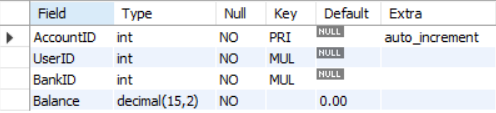
\includegraphics[width=0.6\textwidth]{figures/describe_bankaccounts.png}
    \caption{MySQL result of \texttt{DESCRIBE BankAccounts}}
    \label{fig:sql-describe-bankaccounts}
\end{figure}

Figure~\ref{fig:sql-describe-bankaccounts} shows the structure of the \texttt{BankAccounts} 
table, including its primary key, foreign key columns, and balance field.

% -------------------------------------------------------------------------
\subsection{Sample Data}
% -------------------------------------------------------------------------

Sample data is inserted through \texttt{database/sample\_data.sql}. This file provides 
representative test records for demonstration and validation. The sample data includes user 
profiles, banks, bank accounts, expense categories, income records, expense records, budget 
settings, budget plans, saving goal categories, saving goals, goal contributions, and 
transaction category rules.

Authentication credentials are initialized separately through the bootstrap authentication 
script instead of being hard-coded in the sample data file. This keeps the sample data useful 
for testing while avoiding fixed authentication secrets inside the SQL seed file.

% -------------------------------------------------------------------------
\subsection{Views}
% -------------------------------------------------------------------------

Reporting views are implemented in \texttt{database/views.sql}. Views simplify complex 
reporting queries by storing reusable \texttt{SELECT} logic in the database layer. This allows 
the backend to retrieve dashboard and report data without rebuilding the same joins and 
aggregations repeatedly.

\footnotesize
\renewcommand{\arraystretch}{1.15}

\begin{longtable}{
    >{\raggedright\arraybackslash}p{0.42\linewidth}
    J{0.48\linewidth}
}
\caption{Database views and their purposes}
\label{tab:views} \\

\toprule
\textbf{View} & \textbf{Purpose} \\
\midrule
\endfirsthead

\caption[]{Database views and their purposes (continued)} \\

\toprule
\textbf{View} & \textbf{Purpose} \\
\midrule
\endhead

\midrule
\multicolumn{2}{r}{\textit{Continued on next page}} \\
\endfoot

\bottomrule
\endlastfoot

\path{vw_total_income_by_user}
& Summarizes total income for each user. \\

\path{vw_total_expense_by_user}
& Summarizes total expenses for each user. \\

\path{vw_monthly_income_expense_net_saving}
& Calculates monthly income, expense, and net saving. \\

\path{vw_category_wise_spending}
& Summarizes spending by expense category. \\

\path{vw_budget_vs_actual_monthly}
& Compares planned budget amounts with actual monthly spending. \\

\path{vw_spending_limit_alerts}
& Returns budget categories that are in warning or exceeded status. \\

\path{vw_account_balance_history}
& Computes chronological account running balances. \\

\path{vw_saving_goal_progress}
& Calculates saving goal progress and remaining amount. \\

\path{vw_smart_budget_overview}
& Provides a monthly overview of budget capacity and budget health. \\

\end{longtable}
\normalsize

The following SQL command was used to verify the budget comparison view:

\begin{lstlisting}[style=sqlstyle]
SELECT *
FROM vw_budget_vs_actual_monthly
LIMIT 10;
\end{lstlisting}

\begin{figure}[H]
    \centering
    \makebox[\textwidth][c]{%
        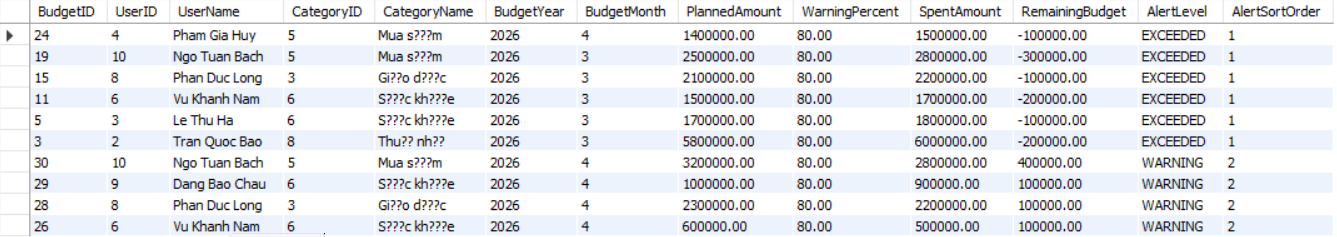
\includegraphics[width=1.05\textwidth]{figures/view_budget_vs_actual.png}
    }
    \caption{MySQL result of \texttt{vw\_budget\_vs\_actual\_monthly}}
    \label{fig:sql-view-budget-vs-actual}
\end{figure}

Figure~\ref{fig:sql-view-budget-vs-actual} shows the result of the budget comparison view. 
The view displays planned amounts, actual spending, remaining budgets, and alert levels for 
monthly budget analysis.

The following SQL command was used to verify the account balance history view:

\begin{lstlisting}[style=sqlstyle]
SELECT *
FROM vw_account_balance_history
LIMIT 10;
\end{lstlisting}

\begin{figure}[H]
    \centering
    \makebox[\textwidth][c]{%
        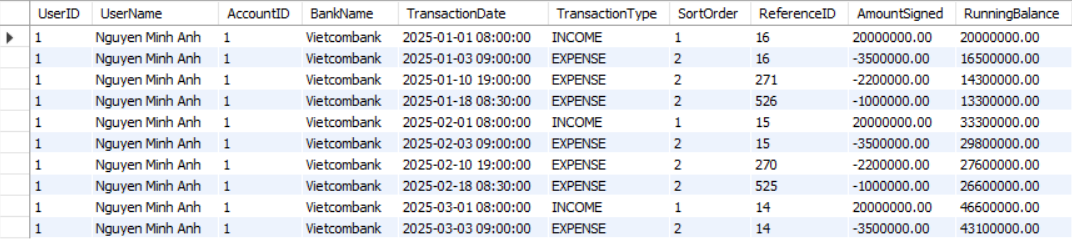
\includegraphics[width=1.05\textwidth]{figures/view_account_balance_history.png}
    }
    \caption{MySQL result of \texttt{vw\_account\_balance\_history}}
    \label{fig:sql-view-account-balance-history}
\end{figure}

Figure~\ref{fig:sql-view-account-balance-history} shows transaction-based running balances for 
a selected account. This view is used to analyze how income and expense transactions change 
account balance over time.

The following SQL command was used to verify the saving goal progress view:

\begin{lstlisting}[style=sqlstyle]
SELECT *
FROM vw_saving_goal_progress
LIMIT 10;
\end{lstlisting}

\begin{figure}[H]
    \centering
    \makebox[\textwidth][c]{%
        \includegraphics[width=1.05\textwidth]{figures/view_saving_goal_progress.png}
    }
    \caption{MySQL result of \texttt{vw\_saving\_goal\_progress}}
    \label{fig:sql-view-saving-goal-progress}
\end{figure}

Figure~\ref{fig:sql-view-saving-goal-progress} shows goal targets, contribution progress, and 
remaining amounts. This view supports the saving goal and debt repayment monitoring workflow.

The following SQL command was used to verify the smart budget overview view:

\begin{lstlisting}[style=sqlstyle]
SELECT *
FROM vw_smart_budget_overview
LIMIT 10;
\end{lstlisting}

\begin{figure}[H]
    \centering
    \makebox[\textwidth][c]{%
        \includegraphics[width=1.05\textwidth]{figures/view_smart_budget_overview.png}
    }
    \caption{MySQL result of \texttt{vw\_smart\_budget\_overview}}
    \label{fig:sql-view-smart-budget-overview}
\end{figure}

Figure~\ref{fig:sql-view-smart-budget-overview} summarizes monthly expected income, fixed 
expenses, available budget capacity, planned budget, and budget health. This view supports the 
smart budget overview shown in the application.

% -------------------------------------------------------------------------
\subsection{Stored Procedures}
% -------------------------------------------------------------------------

Stored procedures are implemented in \texttt{database/procedures.sql}. They centralize common 
write and summary operations, such as adding income, adding expenses, updating transactions, 
deleting transactions, managing budget plans, and generating monthly financial summaries.

\footnotesize
\renewcommand{\arraystretch}{1.15}

\begin{longtable}{
    >{\raggedright\arraybackslash}p{0.38\linewidth}
    J{0.52\linewidth}
}
\caption{Stored procedures and their purposes}
\label{tab:procedures} \\

\toprule
\textbf{Procedure} & \textbf{Purpose} \\
\midrule
\endfirsthead

\caption[]{Stored procedures and their purposes (continued)} \\

\toprule
\textbf{Procedure} & \textbf{Purpose} \\
\midrule
\endhead

\midrule
\multicolumn{2}{r}{\textit{Continued on next page}} \\
\endfoot

\bottomrule
\endlastfoot

\path{sp_add_income}
& Inserts a new income transaction. \\

\path{sp_add_expense}
& Inserts a new expense transaction. \\

\path{sp_update_income}
& Updates an existing income transaction. \\

\path{sp_update_expense}
& Updates an existing expense transaction. \\

\path{sp_delete_income}
& Deletes an income transaction. \\

\path{sp_delete_expense}
& Deletes an expense transaction. \\

\path{sp_add_budget_plan}
& Creates a category-based monthly budget plan. \\

\path{sp_update_budget_plan}
& Updates an existing budget plan. \\

\path{sp_monthly_closure_summary}
& Returns total income, total expense, and net saving for a selected month. \\

\end{longtable}
\normalsize

The following SQL command was used to test the monthly summary stored procedure:

\begin{lstlisting}[style=sqlstyle]
CALL sp_monthly_closure_summary(2025, 4);
\end{lstlisting}

\begin{figure}[H]
    \centering
    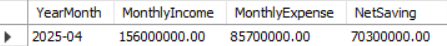
\includegraphics[width=0.6\textwidth]{figures/procedure_monthly_closure.png}
    \caption{MySQL result of executing \texttt{sp\_monthly\_closure\_summary}}
    \label{fig:sql-procedure-monthly-closure}
\end{figure}

Figure~\ref{fig:sql-procedure-monthly-closure} shows that the stored procedure returns monthly 
income, monthly expense, and net saving for the selected period.

% -------------------------------------------------------------------------
\subsection{User-Defined Functions}
% -------------------------------------------------------------------------

User-defined functions are implemented in \texttt{database/functions.sql}. These functions 
provide reusable financial calculations that can be used by reports, queries, procedures, or 
testing scripts.

\footnotesize
\renewcommand{\arraystretch}{1.15}

\begin{longtable}{
    >{\raggedright\arraybackslash}p{0.42\linewidth}
    J{0.48\linewidth}
}
\caption{User-defined functions and their purposes}
\label{tab:functions} \\

\toprule
\textbf{Function} & \textbf{Purpose} \\
\midrule
\endfirsthead

\caption[]{User-defined functions and their purposes (continued)} \\

\toprule
\textbf{Function} & \textbf{Purpose} \\
\midrule
\endhead

\midrule
\multicolumn{2}{r}{\textit{Continued on next page}} \\
\endfoot

\bottomrule
\endlastfoot

\path{fn_total_income_by_user}
& Calculates total income for a user. \\

\path{fn_total_expense_by_user}
& Calculates total expenses for a user. \\

\path{fn_net_saving_by_user}
& Calculates net saving as total income minus total expense. \\

\path{fn_calculated_balance_by_account}
& Calculates transaction-derived balance for a specific account. \\

\end{longtable}
\normalsize

The following SQL command was used to test the user-defined financial functions:

\begin{lstlisting}[style=sqlstyle]
SELECT 
    fn_total_income_by_user(1) AS TotalIncome,
    fn_total_expense_by_user(1) AS TotalExpense,
    fn_net_saving_by_user(1) AS NetSaving;
\end{lstlisting}

\begin{figure}[H]
    \centering
    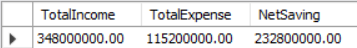
\includegraphics[width=0.6\textwidth]{figures/function_financial_summary.png}
    \caption{MySQL result of user-defined financial functions}
    \label{fig:sql-function-financial-summary}
\end{figure}

Figure~\ref{fig:sql-function-financial-summary} shows that the financial functions correctly 
return total income, total expense, and net saving for a selected user.

% -------------------------------------------------------------------------
\subsection{Triggers}
\label{sec:triggers}
% -------------------------------------------------------------------------

Triggers are implemented in \texttt{database/triggers.sql}. They automatically keep 
\texttt{BankAccounts.Balance} synchronized with income and expense transactions. The database 
defines triggers for \texttt{INSERT}, \texttt{UPDATE}, and \texttt{DELETE} operations on both 
\texttt{Income} and \texttt{Expenses}. It also includes validation triggers to prevent expense 
transactions when the selected account does not have enough balance.

\footnotesize
\renewcommand{\arraystretch}{1.15}

\begin{longtable}{
    >{\raggedright\arraybackslash}p{0.44\linewidth}
    >{\centering\arraybackslash}p{0.12\linewidth}
    J{0.34\linewidth}
}
\caption{Triggers and their execution context}
\label{tab:triggers} \\

\toprule
\textbf{Trigger Name} & \textbf{Timing} & \textbf{Effect} \\
\midrule
\endfirsthead

\caption[]{Triggers and their execution context (continued)} \\

\toprule
\textbf{Trigger Name} & \textbf{Timing} & \textbf{Effect} \\
\midrule
\endhead

\midrule
\multicolumn{3}{r}{\textit{Continued on next page}} \\
\endfoot

\bottomrule
\endlastfoot

\path{trg_expenses_before_insert_check_balance}
& \texttt{BEFORE INSERT}
& Rejects an expense if the selected account is invalid or has insufficient balance. \\

\path{trg_expenses_before_update_check_balance}
& \texttt{BEFORE UPDATE}
& Validates available balance before an expense update is applied. \\

\path{trg_income_after_insert_update_balance}
& \texttt{AFTER INSERT}
& Adds \texttt{NEW.Amount} to the related account balance. \\

\path{trg_income_after_update_update_balance}
& \texttt{AFTER UPDATE}
& Applies the income difference \texttt{NEW.Amount - OLD.Amount}. \\

\path{trg_income_after_delete_update_balance}
& \texttt{AFTER DELETE}
& Subtracts \texttt{OLD.Amount} from the related account balance. \\

\path{trg_expenses_after_insert_update_balance}
& \texttt{AFTER INSERT}
& Subtracts \texttt{NEW.Amount} from the related account balance. \\

\path{trg_expenses_after_update_update_balance}
& \texttt{AFTER UPDATE}
& Adjusts the balance according to the updated expense amount. \\

\path{trg_expenses_after_delete_update_balance}
& \texttt{AFTER DELETE}
& Adds \texttt{OLD.Amount} back to the related account balance. \\

\end{longtable}
\normalsize

The following SQL commands were used to verify the income insert trigger. First, the account 
balance was checked. Then, a test income transaction was inserted. Finally, the account balance 
was checked again.

\begin{lstlisting}[style=sqlstyle]
SELECT AccountID, UserID, Balance AS BalanceBefore
FROM BankAccounts
WHERE UserID = 1 AND AccountID = 1;

INSERT INTO Income (UserID, AccountID, Amount, IncomeDate, Description)
VALUES (1, 1, 123456.00, NOW(), 'Trigger test income');

SELECT AccountID, UserID, Balance AS BalanceAfter
FROM BankAccounts
WHERE UserID = 1 AND AccountID = 1;
\end{lstlisting}

\begin{figure}[H]
    \centering

    \begin{subfigure}[t]{0.75\textwidth}
        \centering
        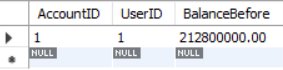
\includegraphics[width=0.5\linewidth]{figures/balance_before_insert.png}
        \caption{Balance before insert}
        \label{fig:trigger-balance-before}
    \end{subfigure}

    \vspace{0.6em}

    \begin{subfigure}[t]{0.75\textwidth}
        \centering
        
\includegraphics[width=1\linewidth]{figures/insert_completed.png}
        \caption{Income inserted}
        \label{fig:trigger-insert-completed}
    \end{subfigure}

    \vspace{0.6em}

    \begin{subfigure}[t]{0.75\textwidth}
        \centering
        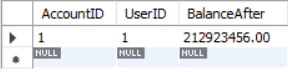
\includegraphics[width=0.5\linewidth]{figures/balance_after_insert.png}
        \caption{Balance after insert}
        \label{fig:trigger-balance-after}
    \end{subfigure}

    \caption{MySQL verification of account balance update after trigger execution}
    \label{fig:sql-trigger-balance-update}
\end{figure}

Figure~\ref{fig:sql-trigger-balance-update} demonstrates that after inserting a new income 
record, the account balance is automatically increased by the trigger. This verifies that 
the database trigger logic keeps account balances synchronized with transaction records.

After the screenshot was captured, the test transaction was removed using the following SQL 
commands to restore the database state:

\begin{lstlisting}[style=sqlstyle]
SELECT IncomeID, UserID, AccountID, Amount, Description
FROM Income
WHERE Description = 'Trigger test income'
ORDER BY IncomeID DESC
LIMIT 1;

DELETE FROM Income
WHERE Description = 'Trigger test income'
ORDER BY IncomeID DESC
LIMIT 1;
\end{lstlisting}

% -------------------------------------------------------------------------
\subsection{Security SQL}
% -------------------------------------------------------------------------

Database-level access control is implemented in \texttt{database/security.sql}. This file 
creates MySQL users that are separate from application-level users stored in \texttt{Users} 
and \texttt{UserCredentials}. This separation allows the system to apply the principle of 
least privilege at the database engine level.

The \texttt{pf\_app} user is intended for backend runtime operations. It is granted 
\texttt{SELECT}, \texttt{INSERT}, \texttt{UPDATE}, \texttt{DELETE}, \texttt{SHOW VIEW}, and 
\texttt{EXECUTE} privileges on the \texttt{Personal\_Finance} database. These privileges allow 
the backend to perform normal application operations while preventing structural operations 
such as \texttt{CREATE TABLE}, \texttt{DROP}, or \texttt{ALTER}.

The following SQL command was used to verify the privileges of the \texttt{pf\_app} user:

\begin{lstlisting}[style=sqlstyle]
SHOW GRANTS FOR 'pf_app'@'%';
\end{lstlisting}

\begin{figure}[H]
    \centering
    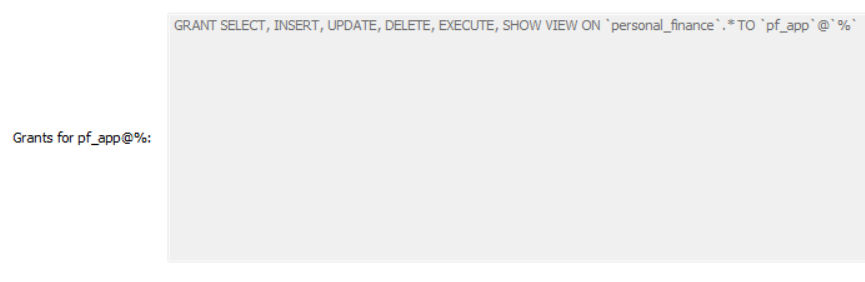
\includegraphics[width=0.7\textwidth]{figures/pf_app_grants.png}
    \caption{MySQL result of database privileges assigned to the \texttt{pf\_app} user}
    \label{fig:sql-pf-app-grants}
\end{figure}

Figure~\ref{fig:sql-pf-app-grants} shows that \texttt{pf\_app} has only the required runtime 
privileges. This verifies that the backend can use a limited database account instead of the 
MySQL root account during normal application execution.

% -------------------------------------------------------------------------
\subsection{Migrations}
% -------------------------------------------------------------------------

The \texttt{database/migrations/} folder is prepared for incremental SQL scripts used to evolve 
the database schema after deployment without discarding existing data. A migration file 
represents a discrete database change, such as adding a new column, creating an index, inserting 
seed data for a new feature, or modifying an existing constraint.

In local development, the database can be rebuilt from the canonical SQL files because no 
production data needs to be preserved. In the Railway cloud deployment, however, rebuilding 
from scratch may destroy live user data. Migrations are therefore the safer mechanism for 
applying database changes to an already-running environment.

% =========================================================
\section{Backend Implementation}
% =========================================================

\subsection{Backend Overview}

The backend of the system is implemented using FastAPI. It provides RESTful API endpoints that connect the frontend application with the MySQL database. The backend is responsible for request validation, authentication, authorization, business logic processing, and database access.

The backend follows a layered architecture. API routers receive requests from the frontend, the service layer handles business rules, and the repository layer communicates with the MySQL database. This structure improves maintainability because API logic, business logic, and SQL operations are separated clearly.

\subsection{Backend Architecture Flow}

Figure~\ref{fig:backend-architecture-flow} shows the main request processing flow in the backend. A request from the frontend is first handled by a FastAPI router. The request is then validated and passed to the service layer. The service layer applies business rules and calls the repository layer to access the database. Finally, the result is returned to the frontend as a JSON response.

\begin{figure}[H]
\centering
\resizebox{0.98\textwidth}{!}{%
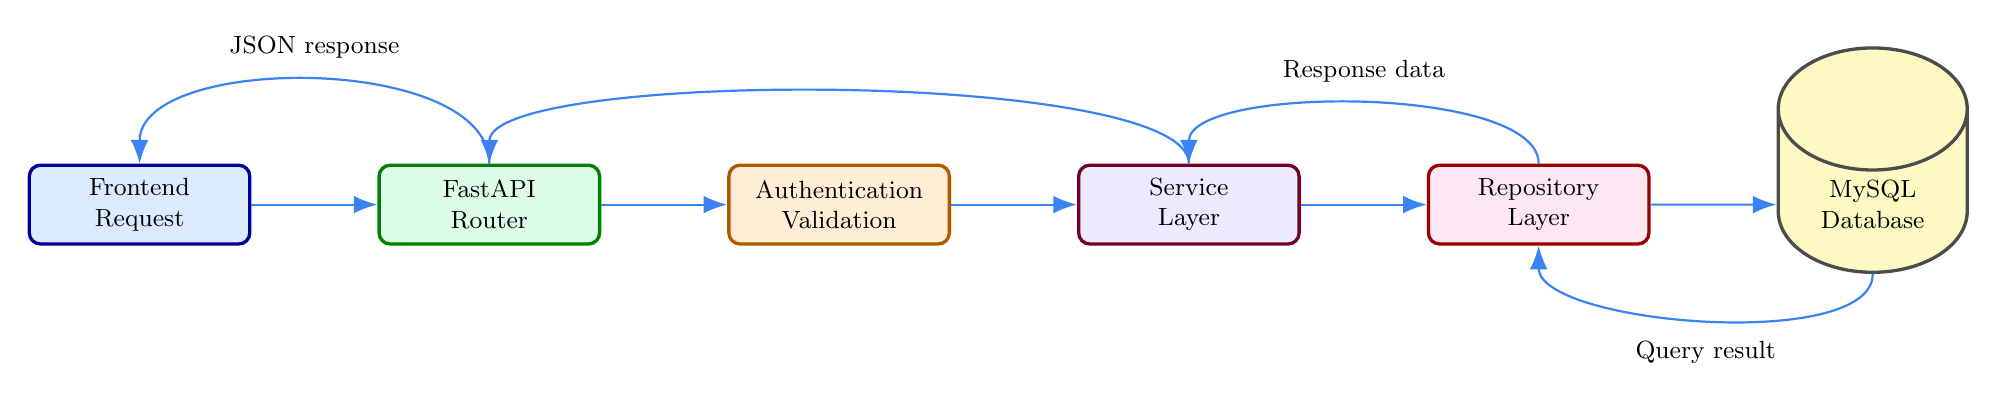
\begin{tikzpicture}[
    node distance=1.6cm,
    every node/.style={font=\small},
    process1/.style={
        rectangle,
        rounded corners,
        draw=blue!60!black,
        very thick,
        align=center,
        minimum width=2.8cm,
        minimum height=1cm,
        fill=softblue
    },
    process2/.style={
        rectangle,
        rounded corners,
        draw=green!50!black,
        very thick,
        align=center,
        minimum width=2.8cm,
        minimum height=1cm,
        fill=softgreen
    },
    process3/.style={
        rectangle,
        rounded corners,
        draw=orange!70!black,
        very thick,
        align=center,
        minimum width=2.8cm,
        minimum height=1cm,
        fill=softorange
    },
    process4/.style={
        rectangle,
        rounded corners,
        draw=purple!60!black,
        very thick,
        align=center,
        minimum width=2.8cm,
        minimum height=1cm,
        fill=softpurple
    },
    process5/.style={
        rectangle,
        rounded corners,
        draw=red!60!black,
        very thick,
        align=center,
        minimum width=2.8cm,
        minimum height=1cm,
        fill=softpink
    },
    database/.style={
        cylinder,
        shape border rotate=90,
        draw=black!70,
        very thick,
        align=center,
        minimum height=1.2cm,
        minimum width=2.4cm,
        fill=softyellow
    },
    arrow/.style={-{Latex[length=3mm]}, thick, draw=lineblue}
]

\node[process1] (frontend) {Frontend\\Request};
\node[process2, right=of frontend] (router) {FastAPI\\Router};
\node[process3, right=of router] (auth) {Authentication\\Validation};
\node[process4, right=of auth] (service) {Service\\Layer};
\node[process5, right=of service] (repo) {Repository\\Layer};
\node[database, right=of repo] (db) {MySQL\\Database};

\draw[arrow] (frontend) -- (router);
\draw[arrow] (router) -- (auth);
\draw[arrow] (auth) -- (service);
\draw[arrow] (service) -- (repo);
\draw[arrow] (repo) -- (db);

\draw[arrow] (db.south) .. controls +(0,-1.0) and +(0,-1.0) .. node[below, yshift=-0.15cm]{Query result} (repo.south);
\draw[arrow] (repo.north) .. controls +(0,1.0) and +(0,1.0) .. node[above, yshift=0.15cm]{Response data} (service.north);
\draw[arrow] (service.north) .. controls +(0,1.2) and +(0,1.2) .. (router.north);
\draw[arrow] (router.north) .. controls +(0,1.4) and +(0,1.4) .. node[above, yshift=0.15cm]{JSON response} (frontend.north);

\end{tikzpicture}
}
\caption{Backend architecture and request processing flow}
\label{fig:backend-architecture-flow}
\end{figure}

\subsection{Main Backend Components}

The backend contains several route groups that support the main features of the system, including authentication, dashboard, transactions, imports, reports, budgets, alerts, goals, and user management. These routers expose API endpoints under the \texttt{/api/v1} prefix.

The service layer coordinates the main business logic of the system. It validates user actions, checks ownership rules, applies financial rules, and prepares response data. For example, when a user creates an expense, the backend checks whether the selected account belongs to the current user and whether the submitted amount is valid.

The repository layer separates database operations from API logic. It executes SQL queries, retrieves data from MySQL tables and views, and returns the results to the service layer. This makes the backend easier to maintain because database access logic is not mixed directly with route handlers.

\subsection{Backend Responsibilities}

The backend supports the following responsibilities:

\begin{itemize}
    \item \textbf{Authentication and authorization:} Handles login, logout, session validation, OTP-based recovery, and role-based access control.
    \item \textbf{Financial operations:} Handles income, expenses, budgets, saving goals, and transaction import workflows.
    \item \textbf{Reporting:} Retrieves dashboard and report data from SQL views and database queries.
    \item \textbf{Validation and error handling:} Handles invalid credentials, expired sessions, unauthorized access, invalid transaction amounts, insufficient balance, duplicate values, and missing records.
\end{itemize}

Overall, the backend acts as the main bridge between the user interface and the database. It ensures that frontend actions are validated, processed, and stored correctly in MySQL.

% =========================================================
\section{Frontend Implementation}
% =========================================================

\subsection{Frontend Overview}

The frontend is implemented using Next.js, TypeScript, and Tailwind CSS. It provides the user interface for the Personal Finance Management System and allows users to interact with the main features of the application, such as authentication, dashboard monitoring, transaction management, budget planning, saving goals, reports, imports, and administrator user management.

The frontend communicates with the FastAPI backend through REST API calls. Data returned from the backend is displayed through pages, forms, tables, cards, progress bars, and charts. Since the detailed user workflow is demonstrated in the project video, this section focuses on the main frontend structure and interaction flow.

\subsection{Frontend Interaction Flow}

Figure~\ref{fig:frontend-interaction-flow} shows how the frontend interacts with the backend and database. Users interact with Next.js pages, which use reusable UI components and API client functions. API requests are sent to the FastAPI backend, and the returned data is rendered back to the interface.

\begin{figure}[H]
\centering
\resizebox{0.98\textwidth}{!}{%
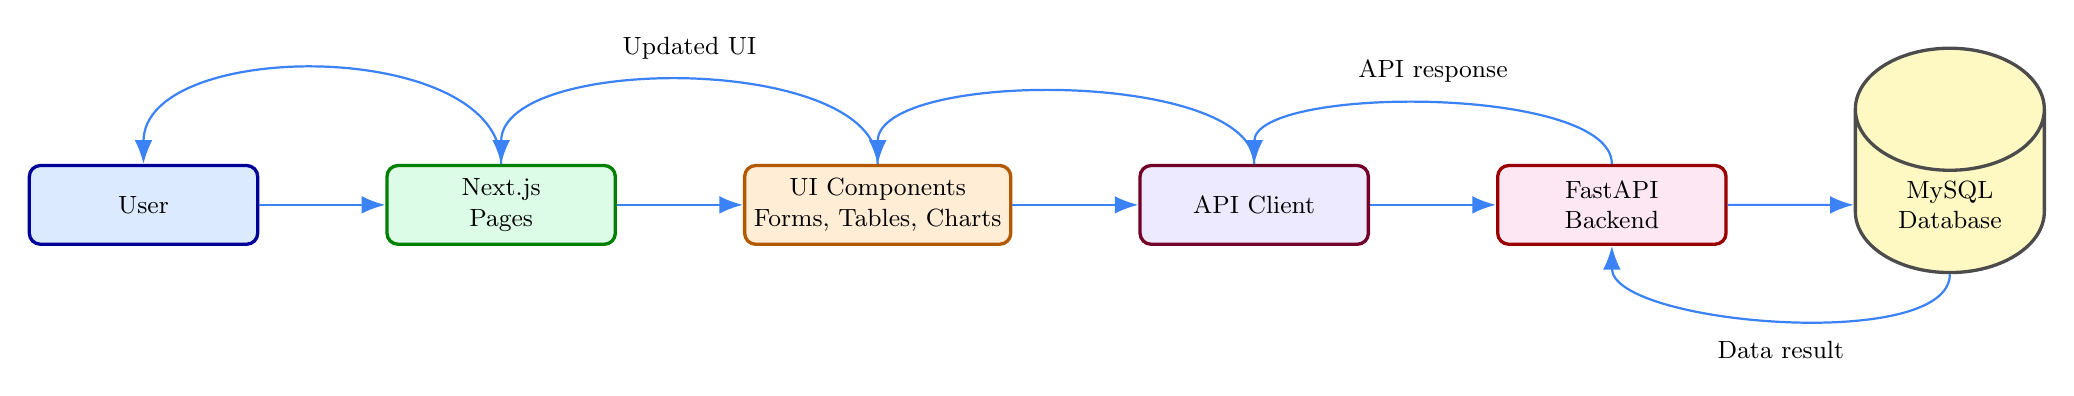
\begin{tikzpicture}[
    node distance=1.6cm,
    every node/.style={font=\small},
    userbox/.style={
        rectangle,
        rounded corners,
        draw=blue!60!black,
        very thick,
        align=center,
        minimum width=2.9cm,
        minimum height=1cm,
        fill=softblue
    },
    pagebox/.style={
        rectangle,
        rounded corners,
        draw=green!50!black,
        very thick,
        align=center,
        minimum width=2.9cm,
        minimum height=1cm,
        fill=softgreen
    },
    uibox/.style={
        rectangle,
        rounded corners,
        draw=orange!70!black,
        very thick,
        align=center,
        minimum width=2.9cm,
        minimum height=1cm,
        fill=softorange
    },
    apibox/.style={
        rectangle,
        rounded corners,
        draw=purple!60!black,
        very thick,
        align=center,
        minimum width=2.9cm,
        minimum height=1cm,
        fill=softpurple
    },
    backendbox/.style={
        rectangle,
        rounded corners,
        draw=red!60!black,
        very thick,
        align=center,
        minimum width=2.9cm,
        minimum height=1cm,
        fill=softpink
    },
    database/.style={
        cylinder,
        shape border rotate=90,
        draw=black!70,
        very thick,
        align=center,
        minimum height=1.2cm,
        minimum width=2.4cm,
        fill=softyellow
    },
    arrow/.style={-{Latex[length=3mm]}, thick, draw=lineblue}
]

\node[userbox] (user) {User};
\node[pagebox, right=of user] (pages) {Next.js\\Pages};
\node[uibox, right=of pages] (components) {UI Components\\Forms, Tables, Charts};
\node[apibox, right=of components] (client) {API Client};
\node[backendbox, right=of client] (backend) {FastAPI\\Backend};
\node[database, right=of backend] (db) {MySQL\\Database};

\draw[arrow] (user) -- (pages);
\draw[arrow] (pages) -- (components);
\draw[arrow] (components) -- (client);
\draw[arrow] (client) -- (backend);
\draw[arrow] (backend) -- (db);

\draw[arrow] (db.south) .. controls +(0,-1.0) and +(0,-1.0) .. node[below, yshift=-0.15cm]{Data result} (backend.south);
\draw[arrow] (backend.north) .. controls +(0,1.0) and +(0,1.0) .. node[above, yshift=0.15cm]{API response} (client.north);
\draw[arrow] (client.north) .. controls +(0,1.2) and +(0,1.2) .. (components.north);
\draw[arrow] (components.north) .. controls +(0,1.4) and +(0,1.4) .. node[above, yshift=0.15cm]{Updated UI} (pages.north);
\draw[arrow] (pages.north) .. controls +(0,1.6) and +(0,1.6) .. (user.north);

\end{tikzpicture}
}
\caption{Frontend interaction and API communication flow}
\label{fig:frontend-interaction-flow}
\end{figure}

\subsection{Main Frontend Features}

The frontend is organized around the main pages of the application. The authentication pages allow users to log in, recover accounts, and manage access. The dashboard page provides a summary of income, expenses, balances, budgets, and saving progress. The transaction page allows users to create, update, delete, and import income or expense records.

The budget page displays monthly budget settings, planned amounts, actual spending, and warning or exceeded statuses. The saving goals page allows users to track long-term saving or debt repayment goals. The reports page presents financial visualizations such as income versus expense, category spending, budget comparison, and balance history. The admin page supports user management for administrator accounts.

\subsection{User Interface Design}

The interface uses cards, forms, tables, progress indicators, and charts to make financial data easier to understand. Forms are used for data input, tables are used for transaction and user lists, and charts are used for reporting and visual analysis.

The frontend is localized in Vietnamese for labels, buttons, messages, date formatting, and currency display. This makes the system easier to use for the intended users. Administrator-only features are separated from normal user features to ensure that role-based access control is reflected in the user interface.

Overall, the frontend provides a clear and practical interface for personal finance tracking. It allows users to interact with the database-backed features through a web application, while the detailed workflow is demonstrated in the accompanying project video.

% =========================================================
\section{Testing and Evaluation}
\label{sec:testing-evaluation}
% =========================================================

\subsection{Testing Objectives}

The purpose of testing is to verify that the Personal Finance Management System works correctly across the database, backend, frontend, and deployment environments. Since the project focuses on database design and implementation, database testing plays an important role in confirming that tables, constraints, views, stored procedures, functions, triggers, and database users work as expected.

The testing process also verifies that the FastAPI backend can communicate with the MySQL database, the frontend can call backend APIs successfully, and the system can run in both local and cloud environments. The detailed frontend workflow is presented in the project demonstration video, while this report focuses on selected testing evidence and system-level verification.

\subsection{Database Testing}

Database testing was performed using MySQL query results. The main objective was to verify that the SQL implementation correctly creates and manages the database objects required by the system.

The database testing covered the following aspects:

\begin{itemize}
    \item \textbf{Table creation:} verifying that all required tables and views are created in the \texttt{Personal\_Finance} database.
    \item \textbf{Table structure:} checking important tables such as \texttt{BankAccounts}, \texttt{Income}, \texttt{Expenses}, and \texttt{Users}.
    \item \textbf{Reporting views:} testing views such as \texttt{vw\_budget\_vs\_actual\_monthly} and \texttt{vw\_account\_balance\_history}.
    \item \textbf{Stored procedures:} executing procedures such as \texttt{sp\_monthly\_closure\_summary}.
    \item \textbf{User-defined functions:} testing financial calculation functions such as \texttt{fn\_total\_income\_by\_user}, \texttt{fn\_total\_expense\_by\_user}, and \texttt{fn\_net\_saving\_by\_user}.
    \item \textbf{Triggers:} verifying that account balances are updated automatically after transaction changes.
    \item \textbf{Database privileges:} checking the privileges assigned to the \texttt{pf\_app} database user.
\end{itemize}

The MySQL query results for these database tests are already presented in the SQL Implementation chapter. Therefore, this chapter does not repeat all database screenshots, but summarizes the testing coverage and focuses on application-level and deployment-level verification.

\subsection{Backend Testing}

Backend testing verifies that the FastAPI application can process requests correctly and return valid responses. The tested backend areas include authentication, transaction management, budget operations, goal management, report generation, import workflow, and administrator user management.

The backend testing focused on the following points:

\begin{itemize}
    \item The backend service starts successfully.
    \item The health check endpoint returns a valid response.
    \item API routes are available through FastAPI Swagger UI.
    \item Protected routes require authentication.
    \item Invalid input is rejected with appropriate error responses.
    \item Backend APIs can retrieve and update data from the MySQL database.
\end{itemize}

The following screenshot shows the backend health check response.

\begin{figure}[H]
    \centering
    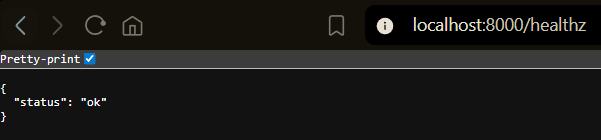
\includegraphics[width=0.85\textwidth]{figures/backend_health_check.png}
    \caption{Backend health check response}
    \label{fig:backend-health-check}
\end{figure}

Figure~\ref{fig:backend-health-check} confirms that the backend service is running and can respond to requests.

The following screenshot shows the FastAPI Swagger UI.

\begin{figure}[H]
    \centering
    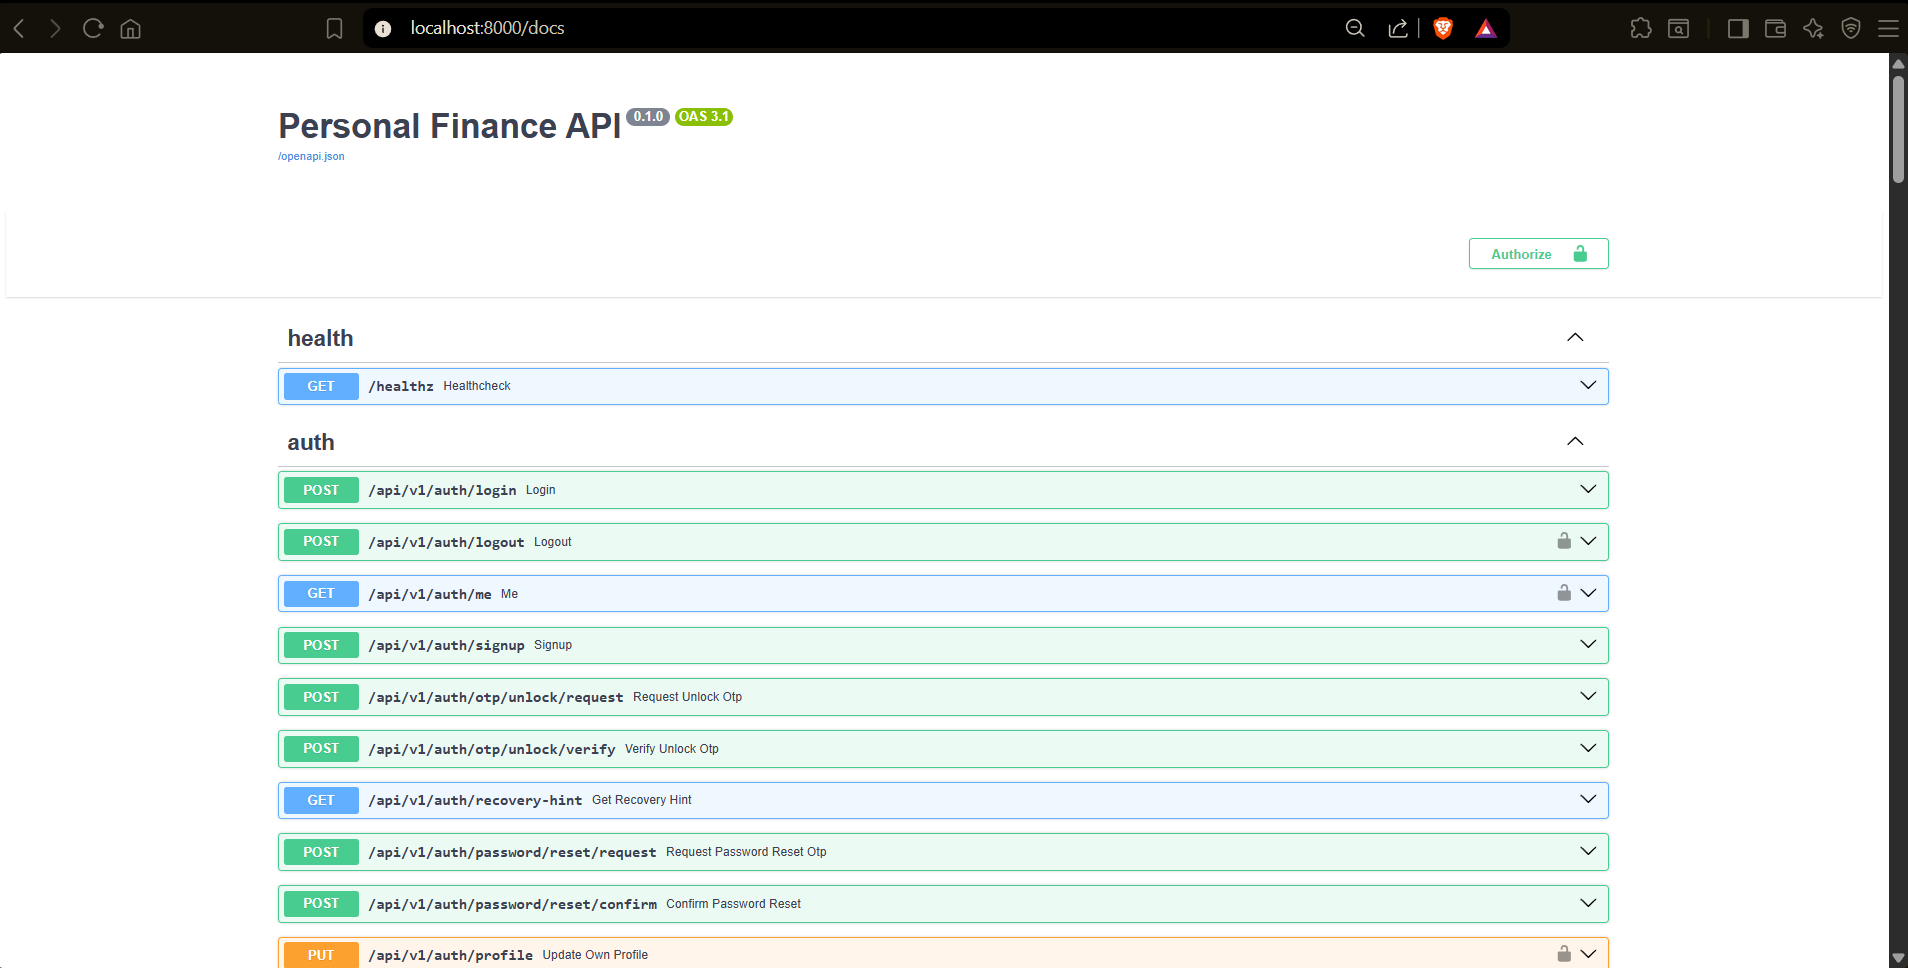
\includegraphics[width=0.95\textwidth]{figures/fastapi_swagger.png}
    \caption{FastAPI Swagger UI showing available backend endpoints}
    \label{fig:fastapi-swagger}
\end{figure}

Figure~\ref{fig:fastapi-swagger} shows the available backend API endpoints. These endpoints support authentication, dashboard data, transactions, budgets, goals, reports, imports, and user management.

\subsection{Frontend Testing}

Frontend testing verifies that the user interface can display data correctly and interact with backend APIs. The main tested workflows include login, dashboard display, transaction management, budget tracking, saving goal monitoring, report visualization, transaction import, and administrator user management.

Since the detailed frontend workflow is shown in the project demonstration video, this report only includes selected frontend evidence. The screenshot below shows the dashboard after a successful login.

\begin{figure}[H]
    \centering
    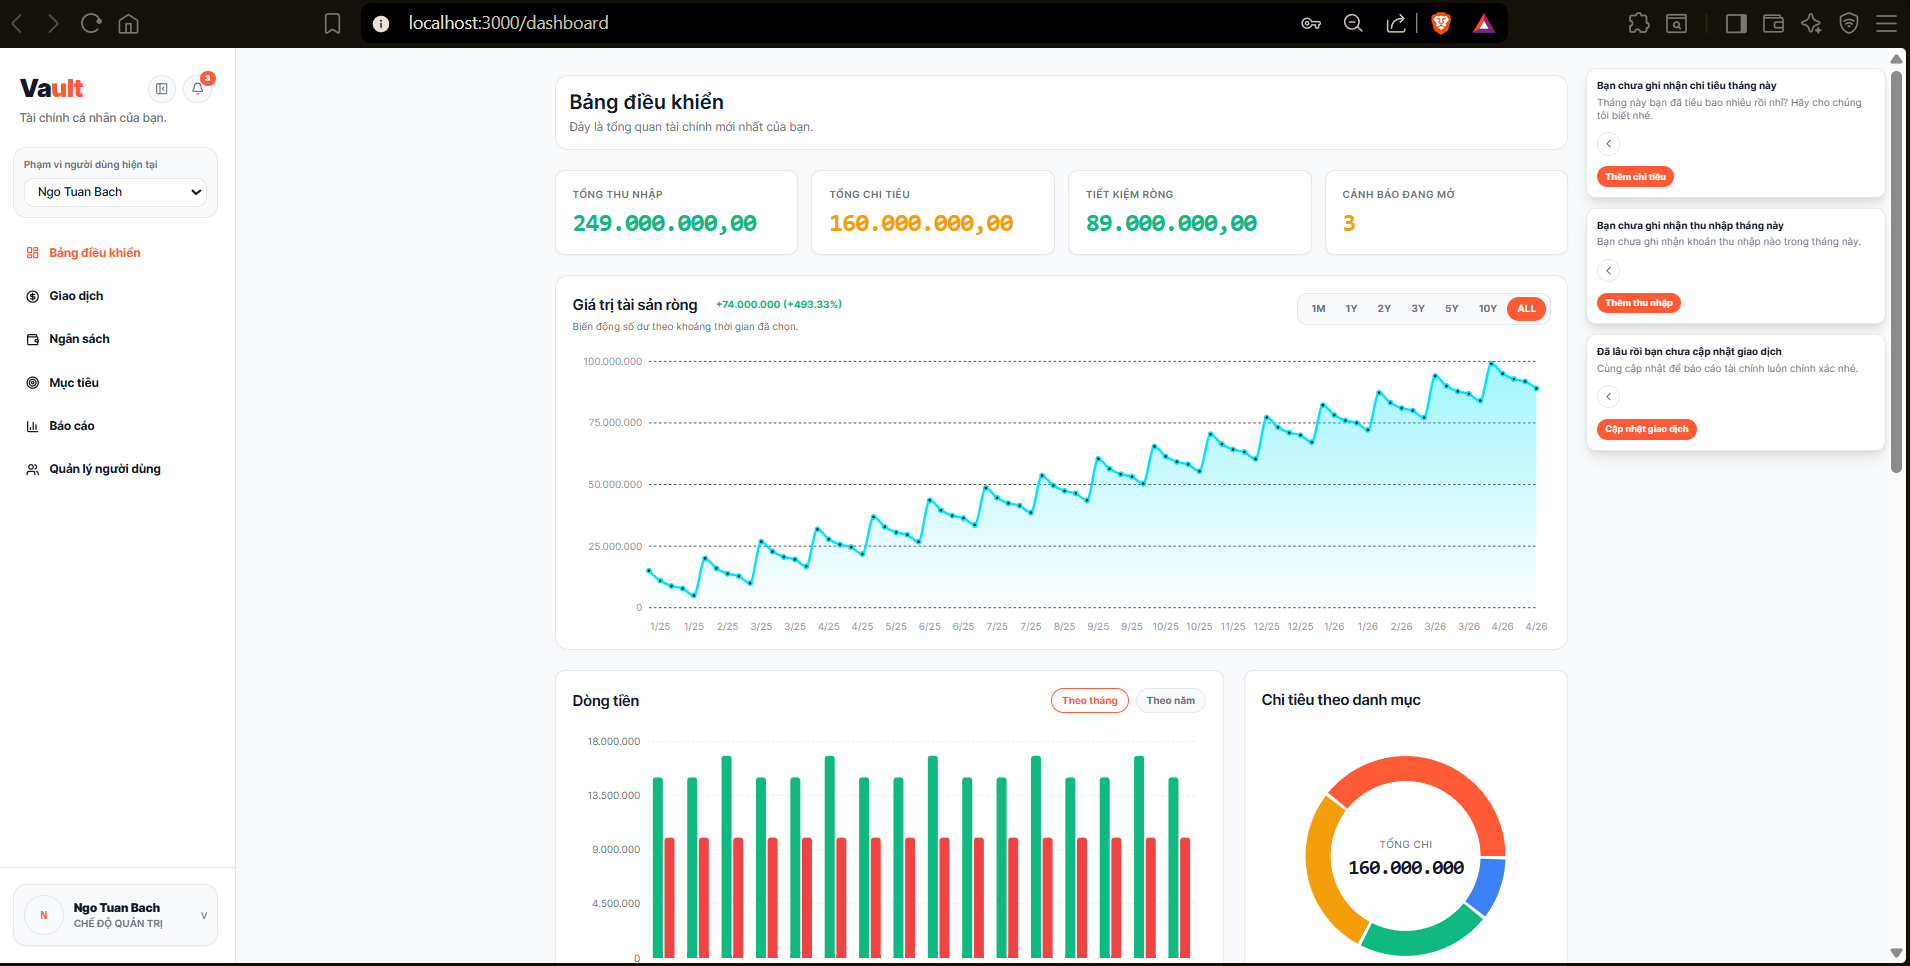
\includegraphics[width=0.95\textwidth]{figures/dashboard_after_login.png}
    \caption{Dashboard page after successful login}
    \label{fig:dashboard-after-login}
\end{figure}

Figure~\ref{fig:dashboard-after-login} confirms that the frontend can authenticate a user, retrieve financial data from the backend, and display summary information on the dashboard.

\subsection{Deployment Testing}

Deployment testing verifies that the system can run in both local and cloud environments. In local development, Docker Compose is used to run the MySQL database, FastAPI backend, and Next.js frontend. In the cloud environment, Railway is used to host the MySQL database, backend service, and frontend service.

The deployment testing focused on the following points:

\begin{itemize}
    \item The MySQL database service starts successfully.
    \item The backend can connect to the MySQL database using environment variables.
    \item The frontend can call the backend API through the configured API URL.
    \item The deployed application can be accessed through the public Railway URL.
    \item Database credentials and runtime configuration are managed through environment variables.
\end{itemize}

Detailed local setup commands, Docker Compose commands, Railway variables, and troubleshooting steps are provided in the project README. This report only summarizes the deployment approach and includes one deployment verification screenshot.

\begin{figure}[H]
    \centering
    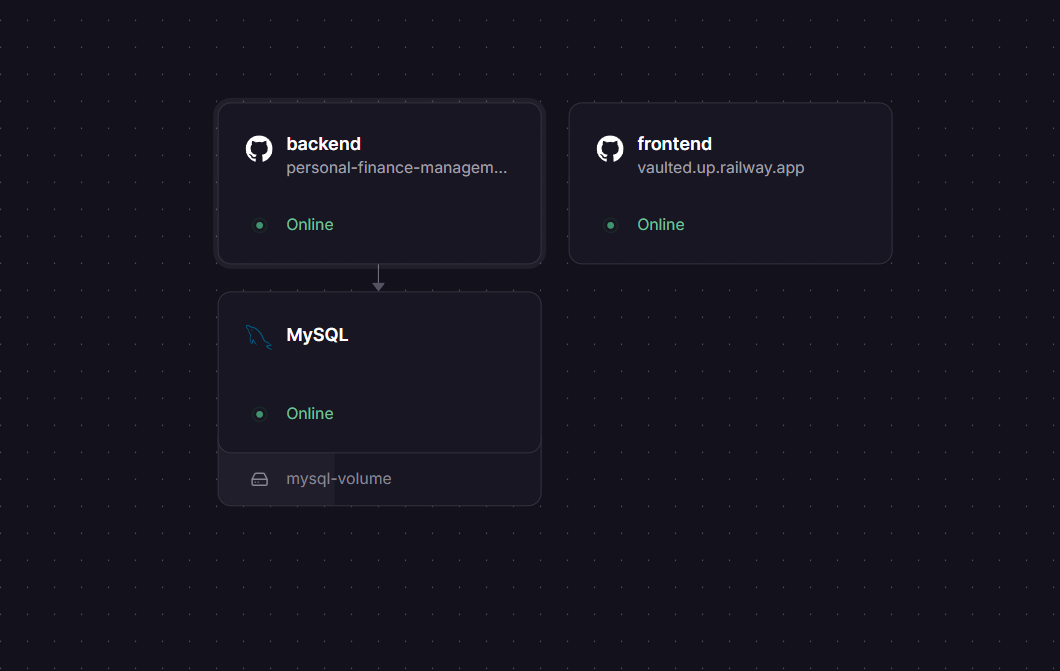
\includegraphics[width=0.8\textwidth]{figures/railway_deployment_status.png}
    \caption{Railway deployment status for frontend, backend, and MySQL services}
    \label{fig:railway-deployment-status}
\end{figure}

Figure~\ref{fig:railway-deployment-status} shows that the required services are deployed successfully on Railway.

\subsection{Test Case Summary}

Table~\ref{tab:test-cases} summarizes the main test cases used to evaluate the system. These test cases cover the most important workflows of the application.

\small
\renewcommand{\arraystretch}{1.2}

\begin{longtable}{
    >{\raggedright\arraybackslash}p{0.24\linewidth}
    J{0.28\linewidth}
    J{0.28\linewidth}
    >{\centering\arraybackslash}p{0.10\linewidth}
}
\caption{Sample test case summary}
\label{tab:test-cases} \\

\toprule
\textbf{Test Case} & \textbf{Input / Action} & \textbf{Expected Result} & \textbf{Status} \\
\midrule
\endfirsthead

\caption[]{Sample test case summary (continued)} \\

\toprule
\textbf{Test Case} & \textbf{Input / Action} & \textbf{Expected Result} & \textbf{Status} \\
\midrule
\endhead

\midrule
\multicolumn{4}{r}{\textit{Continued on next page}} \\
\endfoot

\bottomrule
\endlastfoot

Admin login 
& Enter valid admin email and password. 
& The user is authenticated and redirected to the dashboard. 
& Pass \\

Invalid login 
& Enter an incorrect password. 
& The login request is rejected and an error message is shown. 
& Pass \\

Add income 
& Submit a valid income transaction. 
& The income record is saved and the selected account balance increases. 
& Pass \\

Add expense 
& Submit a valid expense transaction. 
& The expense record is saved and the selected account balance decreases. 
& Pass \\

Insufficient balance 
& Submit an expense amount greater than the account balance. 
& The transaction is rejected by the system. 
& Pass \\

Update transaction 
& Edit an existing income or expense transaction. 
& The transaction and account balance are updated correctly. 
& Pass \\

Delete transaction 
& Delete an existing income or expense transaction. 
& The transaction is removed and the account balance is adjusted. 
& Pass \\

Budget warning 
& Spending reaches the warning threshold. 
& The budget warning status is displayed. 
& Pass \\

Budget exceeded 
& Spending exceeds the planned budget amount. 
& The exceeded status is displayed. 
& Pass \\

Goal contribution 
& Add a contribution to an active saving goal. 
& The goal progress is updated correctly. 
& Pass \\

Transaction import 
& Upload and confirm a valid CSV or Excel file. 
& The transaction rows are parsed, previewed, and imported. 
& Pass \\

Report display 
& Open the reports page. 
& Financial charts and summaries are displayed correctly. 
& Pass \\

Admin user management 
& Update a user's role or account status. 
& The user information is updated correctly. 
& Pass \\

Railway deployment 
& Open the deployed application URL. 
& The frontend, backend, and MySQL services work together successfully. 
& Pass \\

\end{longtable}
\normalsize

\subsection{Evaluation}

The testing results show that the system satisfies the main functional requirements. Users can log in, manage income and expense transactions, track account balances, configure budgets, monitor saving goals, import transaction files, and view financial reports. Administrator-level user management is also supported.

At the database level, MySQL testing confirms that tables, constraints, views, stored procedures, user-defined functions, triggers, and database privileges work correctly. The trigger tests confirm that account balances are synchronized with transaction changes, while the view and function tests confirm that financial summaries can be calculated at the database layer.

At the application level, backend and frontend testing confirm that the FastAPI backend can communicate with MySQL and that the Next.js frontend can retrieve and display financial data through API calls. Deployment testing confirms that the system can run locally through Docker Compose and globally through Railway.

Overall, the system is functional, testable, and suitable for the intended purpose of personal finance management.

% =========================================================
\section{Discussion}
\label{sec:discussion}
% =========================================================

\subsection{Security and Data Integrity Summary}

Security and data integrity are important aspects of the system because the application stores personal financial information. At the application level, user authentication is handled through password hashing, session tokens, OTP-based account recovery, and role-based access control. Passwords, OTP codes, and session tokens are not stored in plain text.

At the database level, the system uses MySQL constraints and security configuration to protect data consistency. Primary keys uniquely identify records, foreign keys enforce relationships between tables, unique constraints prevent duplicate important values, and check constraints validate financial amounts and period values. Triggers are used to keep account balances synchronized when income or expense records change.

The system also applies the principle of least privilege at the database level. The \texttt{pf\_app} database user is intended for backend runtime operations and receives only the required permissions, such as \texttt{SELECT}, \texttt{INSERT}, \texttt{UPDATE}, \texttt{DELETE}, \texttt{SHOW VIEW}, and \texttt{EXECUTE}. This avoids using the MySQL root account for normal application execution.

\subsection{Achievements}

The project successfully implements a database-backed personal finance management system. The main achievements include:

\begin{itemize}
    \item A normalized MySQL database schema for users, accounts, transactions, budgets, goals, authentication, imports, and reporting.
    \item Core ERD and supporting ERDs for authentication/security and transaction import/linking.
    \item SQL implementation with tables, constraints, indexes, views, stored procedures, user-defined functions, triggers, and security users.
    \item A FastAPI backend that exposes RESTful API endpoints and connects the frontend to the database.
    \item A Next.js frontend that provides user-facing pages for dashboard, transactions, budgets, goals, reports, imports, and admin management.
    \item Local deployment using Docker Compose and cloud deployment using Railway.
    \item Testing evidence through MySQL query results, backend API verification, frontend workflow testing, and deployment verification.
\end{itemize}

These achievements show that the project meets the main requirements of a database management system project and demonstrates practical use of relational database design and SQL implementation.

\subsection{Limitations}

Although the system is functional, it still has several limitations. First, the system does not connect directly to real banking APIs. Bank accounts in the system are internal records created by users, and transactions are entered manually or imported from files. Second, the transaction import feature depends on the format and quality of the uploaded CSV or Excel file. If the file structure is inconsistent, additional preprocessing may be required.

The current system also focuses mainly on rule-based reporting and visualization. It does not include advanced predictive analytics, automated spending recommendations, or AI-based financial planning. In addition, the system is implemented as a web application and does not yet provide a dedicated mobile application.

\subsection{Future Improvements}

Future improvements can extend the system in several directions:

\begin{itemize}
    \item Integrate with real banking APIs to automatically import transactions.
    \item Add recurring transaction support for rent, subscriptions, salaries, and fixed expenses.
    \item Improve transaction import by supporting more file formats and smarter column mapping.
    \item Add notifications for budget warnings, goal deadlines, and unusual spending patterns.
    \item Implement AI-based spending prediction and cash flow forecasting.
    \item Add export features for PDF and Excel financial reports.
    \item Develop a mobile application for easier personal finance tracking.
    \item Improve admin monitoring and audit log visualization.
\end{itemize}

These improvements would make the system more automated, intelligent, and suitable for long-term personal finance management.

% =========================================================
\section{Conclusion}
\label{sec:conclusion}
% =========================================================

This project developed a Personal Finance Management System using MySQL, FastAPI, and Next.js. The main objective of the system is to help users manage their personal financial data, including bank accounts, income, expenses, budgets, saving goals, transaction imports, reports, and authentication-related information.

From the database perspective, the project successfully designed and implemented a relational database named \texttt{Personal\_Finance}. The database design includes a Core ERD for the main financial entities, an Authentication and Security Supporting ERD, and a Transaction Import and Linking Supporting ERD. These ERDs show how the system organizes financial records, authentication data, import workflows, and goal-related transactions.

The SQL implementation demonstrates the use of important database management concepts. The schema defines tables, primary keys, foreign keys, unique constraints, check constraints, and indexes. Views are used to simplify reporting queries, stored procedures are used to centralize common database operations, user-defined functions are used for reusable financial calculations, and triggers are used to keep account balances synchronized with income and expense transactions. The \texttt{security.sql} file also introduces database-level users such as \texttt{pf\_app} and \texttt{pf\_readonly}, supporting the principle of least privilege.

The backend implementation uses FastAPI to provide RESTful APIs between the frontend and the MySQL database. It handles authentication, validation, business logic, financial operations, reporting, import processing, and admin user management. The frontend implementation uses Next.js, TypeScript, and Tailwind CSS to provide a web interface for users to interact with the system. The web interface supports dashboard monitoring, transaction management, budget planning, saving goal tracking, reports, import preview, and admin management.

Testing confirmed that the system works correctly across the database, backend, frontend, and deployment environments. MySQL query results verified the creation of tables, views, stored procedures, functions, triggers, and database privileges. Backend testing confirmed that API endpoints are available and functional. Frontend testing confirmed that users can complete the main workflows through the web interface. Deployment testing confirmed that the system can run locally using Docker Compose and globally using Railway.

Overall, the project achieved its main goals and demonstrates a complete database-backed application. It applies relational database design principles, implements advanced SQL objects, connects the database with a backend API, and provides a practical frontend for personal finance management. Although the system does not yet integrate with real banking APIs or advanced prediction features, it provides a solid foundation for future improvements such as automated bank synchronization, recurring transactions, spending prediction, notifications, and mobile support.

\newpage
% =========================================================
\phantomsection
\addcontentsline{toc}{section}{References}
% =========================================================

\begin{thebibliography}{99}

\bibitem{mysql}
Oracle Corporation.
\newblock \textit{MySQL 8.4 Reference Manual}.
\newblock Available at: \url{https://dev.mysql.com/doc/}

\bibitem{fastapi}
FastAPI.
\newblock \textit{FastAPI Documentation}.
\newblock Available at: \url{https://fastapi.tiangolo.com/}

\bibitem{nextjs}
Vercel.
\newblock \textit{Next.js Documentation}.
\newblock Available at: \url{https://nextjs.org/docs}

\bibitem{react}
Meta Open Source.
\newblock \textit{React Documentation}.
\newblock Available at: \url{https://react.dev/}

\bibitem{tailwind}
Tailwind Labs.
\newblock \textit{Tailwind CSS Documentation}.
\newblock Available at: \url{https://tailwindcss.com/docs}

\bibitem{docker}
Docker Inc.
\newblock \textit{Docker Documentation}.
\newblock Available at: \url{https://docs.docker.com/}

\bibitem{railway}
Railway.
\newblock \textit{Railway Documentation}.
\newblock Available at: \url{https://docs.railway.com/}

\bibitem{mysqlconnector}
Oracle Corporation.
\newblock \textit{MySQL Connector/Python Developer Guide}.
\newblock Available at: \url{https://dev.mysql.com/doc/connector-python/en/}

\bibitem{recharts}
Recharts.
\newblock \textit{Recharts Documentation}.
\newblock Available at: \url{https://recharts.org/}

\bibitem{owasp}
OWASP Foundation.
\newblock \textit{OWASP Authentication Cheat Sheet}.
\newblock Available at: \url{https://cheatsheetseries.owasp.org/cheatsheets/Authentication_Cheat_Sheet.html}

\bibitem{githubrepo}
Ngo Tuan Bach.
\newblock \textit{Personal Finance Management System Repository}.
\newblock Available at: \url{\repoURL}

\end{thebibliography}
\newpage
% =========================================================
% APPENDIX
% =========================================================
\clearpage
\appendix

\phantomsection
\section*{Appendix}
\addcontentsline{toc}{section}{Appendix}

% =========================================================
\section{Source Code Structure}
\label{appendix:source-code-structure}
% =========================================================
\begin{lstlisting}[style=codestyle, caption={Project source code structure}]
Personal-Finance-management/
  database/
    schema.sql
    sample_data.sql
    views.sql
    procedures.sql
    functions.sql
    triggers.sql
    security.sql
    migrations/

  backend/
    app/
      main.py
      config.py
      deps.py
      routers/

  frontend/
    src/
      app/
      components/
      lib/
      providers/
      types/

  python_app/
    services/
    repositories/
    db_connection.py

  ops/
    bootstrap_auth.py
    docker/
      reset_database.sh
      apply_views.sh

  docs/
    assignment files
    report files
    ERD images
\end{lstlisting}

% =========================================================
\section{SQL Script Inventory}
\label{appendix:sql-script-inventory}
% =========================================================
\small
\renewcommand{\arraystretch}{1.2}

\begin{longtable}{
    >{\raggedright\arraybackslash}p{0.30\linewidth}
    J{0.60\linewidth}
}
\caption{SQL script inventory}
\label{tab:sql-script-inventory} \\

\toprule
\textbf{SQL File} & \textbf{Purpose} \\
\midrule
\endfirsthead

\caption[]{SQL script inventory (continued)} \\

\toprule
\textbf{SQL File} & \textbf{Purpose} \\
\midrule
\endhead

\midrule
\multicolumn{2}{r}{\textit{Continued on next page}} \\
\endfoot

\bottomrule
\endlastfoot

\texttt{schema.sql} 
& Creates the \texttt{Personal\_Finance} database, tables, primary keys, foreign keys, unique constraints, check constraints, and indexes. \\

\texttt{sample\_data.sql} 
& Inserts representative sample data for users, banks, bank accounts, transactions, budgets, saving goals, goal contributions, and category rules. \\

\texttt{views.sql} 
& Creates reporting and dashboard views such as budget comparison, account balance history, category-wise spending, and saving goal progress. \\

\texttt{procedures.sql} 
& Creates stored procedures for income, expense, budget, and monthly financial summary operations. \\

\texttt{functions.sql} 
& Creates user-defined functions for reusable financial calculations such as total income, total expense, net saving, and account balance calculation. \\

\texttt{triggers.sql} 
& Creates triggers that automatically update account balances and prevent invalid expense transactions when the selected account has insufficient balance. \\

\texttt{security.sql} 
& Defines database-level MySQL users and privileges, including limited runtime access for \texttt{pf\_app} and read-only access for \texttt{pf\_readonly}. \\

\texttt{migrations/} 
& Contains or prepares incremental SQL scripts for updating an existing database without resetting all data. \\

\end{longtable}
\normalsize

% =========================================================
\section{Full ERD}
\label{appendix:full-erd}
% =========================================================

\begin{figure}[H]
    \centering
    \makebox[\textwidth][c]{%
        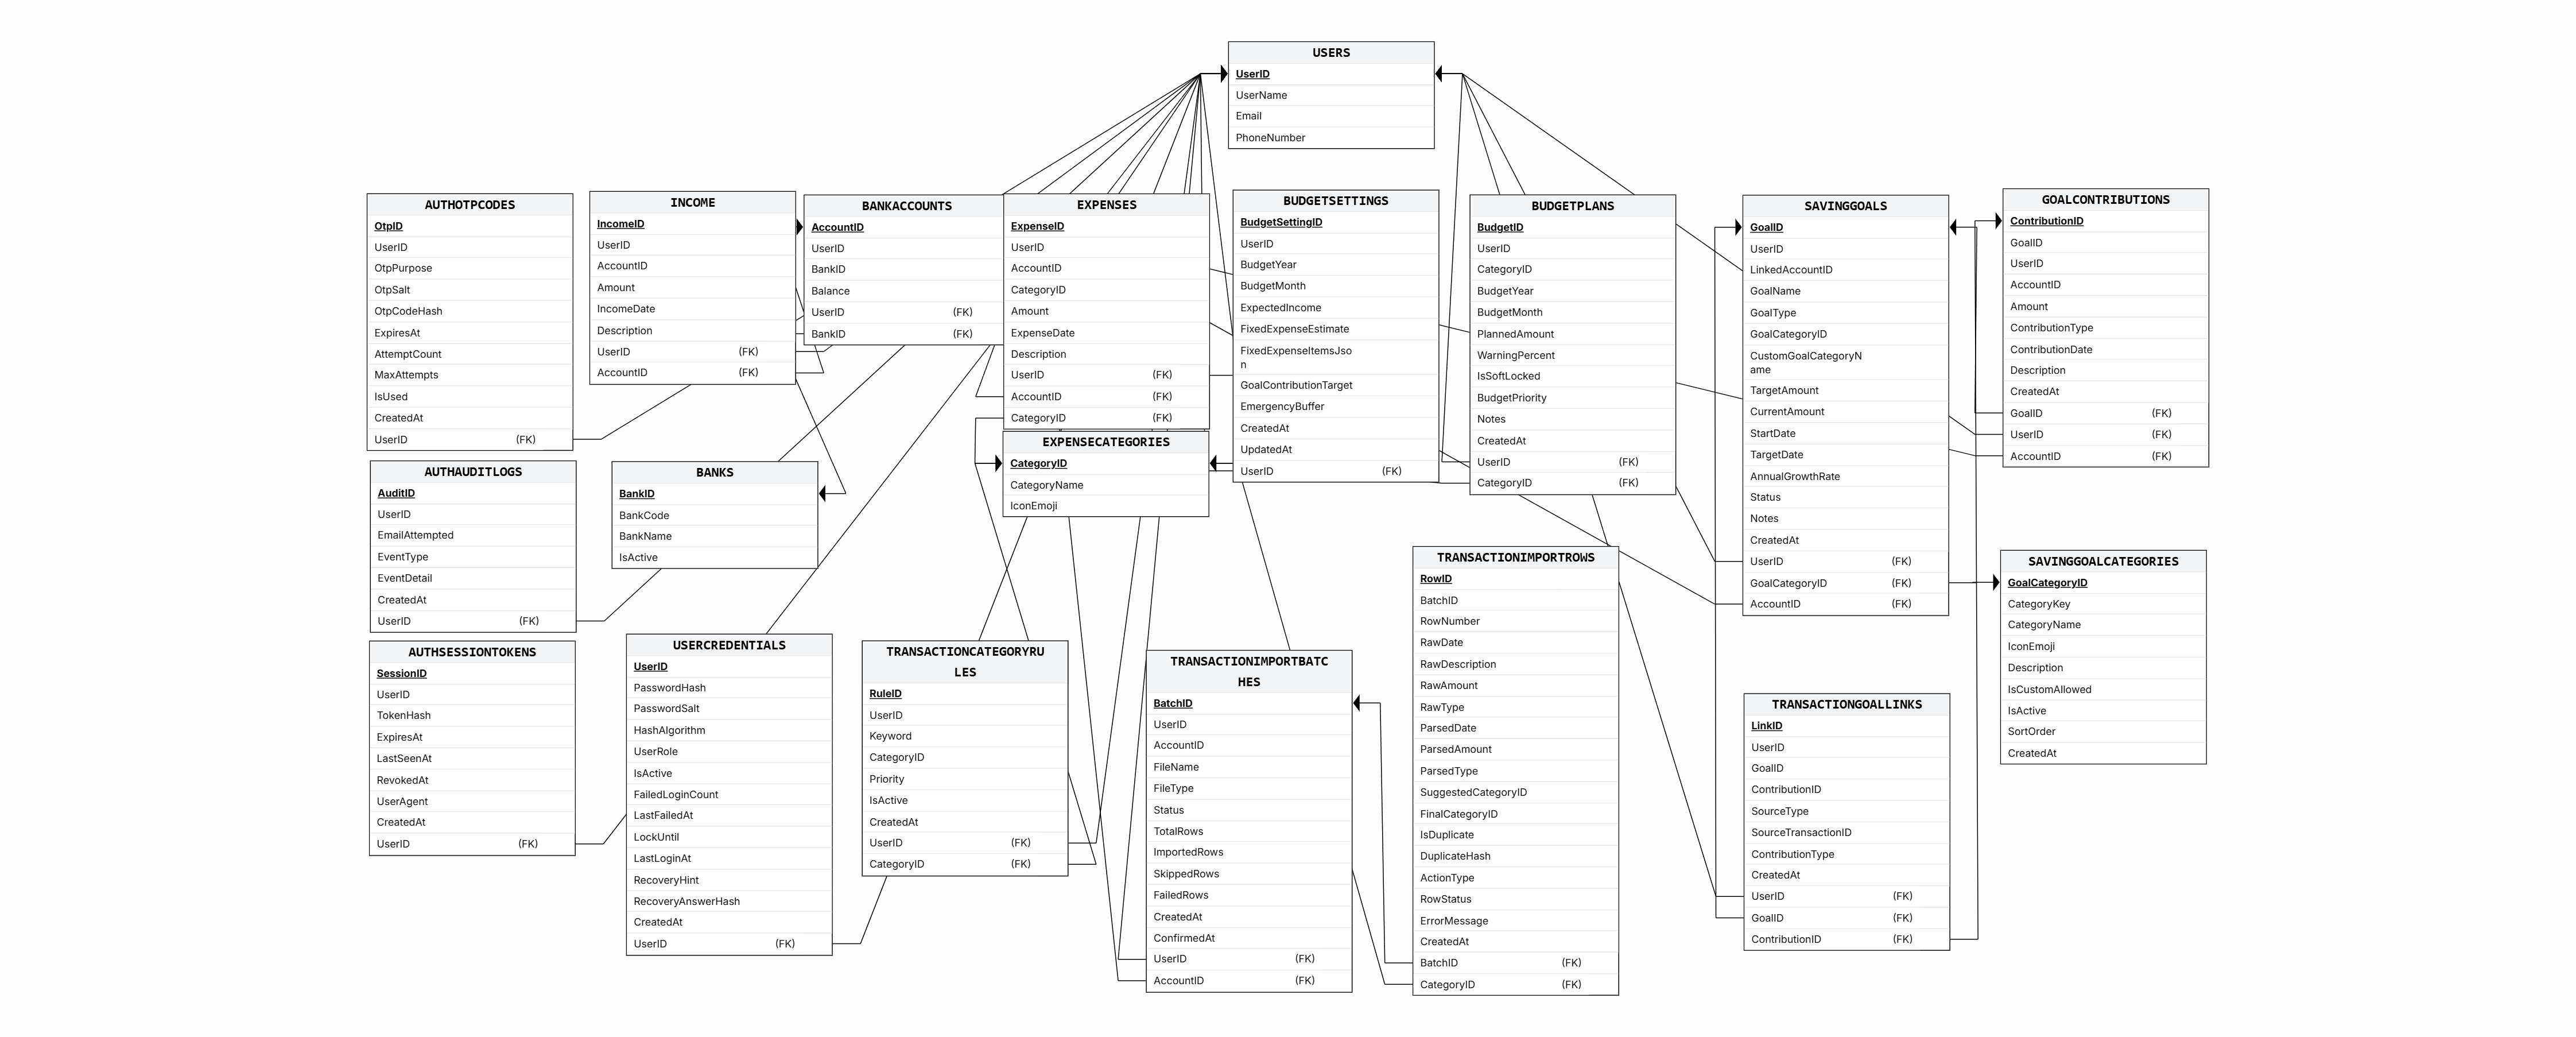
\includegraphics[width=1.5\textwidth]{ERD/full_erd.png}
    }
    \caption{Full ERD of the \dbname{} database}
    \label{fig:appendix-full-erd}
\end{figure}

% =========================================================
\section{Repository and Demo Links}
\label{appendix:repository-demo-links}
% =========================================================

\begin{itemize}
    \item GitHub Repository: \url{\repoURL}
    \item Demo Video: \url{\demoURL}
    \item Deployed Website: \url{\frontendURL}
\end{itemize}

\end{document}
